\documentclass[aps,prb,twocolumn,superscriptaddress,longbibliography,floatfix]{revtex4-2}
\usepackage{amsmath,amssymb,amsthm}
\usepackage{graphicx}
\usepackage{capt-of}
\graphicspath{{figures/}{technical_report/figures/}}
\usepackage[colorlinks=true,urlcolor=blue,linkcolor=blue,citecolor=blue]{hyperref}
\usepackage[dvipsnames]{xcolor}
\usepackage{bm}
\usepackage{soul}
\usepackage{pifont}
\usepackage{mathtools}
\usepackage{tikz}
\usetikzlibrary{tikzmark,arrows.meta,positioning,shapes.geometric,calc}
\usepackage{array}
\usepackage[normalem]{ulem}
\usepackage{mdframed}
\usepackage{enumitem}
\usepackage{makecell}
\usepackage{physics}
\usepackage{comment}

\DeclareMathOperator\arctanh{arctanh}
\DeclareMathOperator{\Sgn}{Sgn}

% ── Shorthands ──
\newcommand{\ii}{\mathrm{i}}
\newcommand{\mc}[1]{\mathcal{#1}}
\newcommand{\mr}[1]{\mathrm{#1}}
\newcommand{\mf}[1]{\mathfrak{#1}}
\newcommand{\mb}[1]{\mathbb{#1}}
\newcommand{\mbf}[1]{\mathbf{#1}}
\newcommand{\bs}[1]{\boldsymbol{#1}}
\newcommand{\h}[1]{\hat{#1}}
\newcommand{\Id}{\mathbf{1}}

% ── Calligraphic / hatted shortcuts ──
\newcommand{\cT}{\mc{T}}
\newcommand{\cC}{\mc{C}}
\newcommand{\cS}{\mc{S}}
\newcommand{\cU}{\mc{U}}
\newcommand{\hcT}{\h{\mc{T}}}
\newcommand{\hcC}{\h{\mc{C}}}
\newcommand{\hcS}{\h{\mc{S}}}
\newcommand{\hcN}{\hat{\mathcal N}}

% ── Physics objects ──
\newcommand{\comp}[1]{\underset{#1}{\bigcirc}}
\newcommand{\bfr}{\boldsymbol r}
\newcommand{\kett}[1]{\ket{#1}\!\rangle}
\newcommand{\braa}[1]{\langle\!\bra{#1}}
\newcommand{\TS}{\kett{\mr{TS}}}
\newcommand{\CI}{\kett{\mr{CI}}}
\newcommand{\vac}{\kett{\mr{vac}}}
\newcommand{\fSWAP}{\operatorname{fSWAP}}
\newcommand{\AZK}[1]{\mc{K}\_{\mr{#1}}}

% ── Check / x marks ──
\newcommand{\cmark}{\textcolor{green}{\ding{51}}}
\newcommand{\xmark}{\textcolor{red}{\ding{55}}}

% ── Draft annotation (single macro per person; all red for submission mode) ──
\newcommand{\drafthighlight}[1]{\textcolor{red}{#1}}
\newcommand{\cmjadd}[1]{\drafthighlight{#1}}
\newcommand{\abadd}[1]{\drafthighlight{#1}}
\newcommand{\HPadd}[1]{\drafthighlight{#1}}
\newcommand{\cmjCom}[1]{\textcolor{red}{[CMJ: #1]}}
\newcommand{\abcom}[1]{\textcolor{purple}{[AB: #1]}}
\newcommand{\HPcom}[1]{\textcolor{cyan}{[HP: #1]}}

% ── Theorem environments ──
\theoremstyle{plain}
\newtheorem{theorem}{Theorem}
\theoremstyle{definition}
\newtheorem{definition}[theorem]{Definition}
\theoremstyle{remark}
\newtheorem{remark}[theorem]{Remark}

\setstcolor{magenta}

\begin{document}

\title{Technical Report}
\author{Asadullah Bhuiyan}
\noaffiliation
\date{\today}

\begin{abstract}
  Details on dynamical preparation of boundary modes.
\end{abstract}

\maketitle

\setcounter{tocdepth}{2}
\tableofcontents

\section{Background}

We consider a 2+1d dynamical quantum system subject to measurements, unitary feedback, and ancillary resets that steer arbitrary initial states toward an ensemble of 2d Chern-insulator states after a transient timescale. The dynamics consist of finite-range measurements and local unitary feedback that correct undesired occupation outcomes for truncated overcomplete Wannier (OW) modes by swapping in modes from an ancillary bath. A parameter $\alpha$ controls the topological phase of the dynamics~\cite{BhuiyanPanJian2026}.

The measurement-feedback schedule is periodic, and the dynamics can be described by a Floquet superoperator $\mathcal F$. The protocol therefore resembles a dynamical error-correction code: measurements are performed according to a fixed schedule, and undesired outcomes are actively corrected~\cite{HastingsHaah2021,AasenHaahLiMong2023}. For this reason, we refer to this non-equilibrium system as a \emph{dynamical Chern insulator}. For finite-range OW truncations, however, the measurements are frustrated and do not possess a common dark state. Instead, the dynamics approach a steady-state ensemble of Chern insulators that is robust to local spacetime perturbations of the circuit.

By introducing a spatially dependent $\alpha$, we can create a topological interface between two distinct phases~\cite{Hatsugai1993,HasanKane2010,QiZhang2011}. We show that the dynamics can prepare a topological boundary mode at the interface and that the mode is robust to local perturbations of the circuit. Furthermore, the domain-wall adaptive circuit shows evidence of chiral, critical, topologically protected boundary modes at the interface, consistent with the expected universal conformal-field-theory description of the boundary physics~\cite{CalabreseCardy2004}. We study the critical phenomena of the steady-state ensemble and its dynamics.

\section{Adaptive Circuit Construction}
\subsection{Parent Hamiltonian and Overcomplete Wannier Functions}
To construct our circuit, we will motivate the adaptive dynamics from a parent Hamiltonian $\hat H_{\mr{CI}}$ whose ground state is the target Chern insulator state $\CI$~\cite{BhuiyanPanJian2026}. In real space, $\hat H_{\mr{CI}} $ describes a non-interacting fermionic system is living on a 2d square lattice with two fermion modes $\hat c_{\bfr,\mu=1,2}$ per unit cell, with the unit-cell coordinate $\bfr=(x,y)\in\mathbb{Z}^2$ being a pair of integers. Thus, in the thermodynamic limit, the momentum-space the momentum-space resolved parent Hamiltonian of the target state $\CI$ is given by
\begin{align}
    \hat H_{\mr{CI}} &= \int\frac{d^2\boldsymbol k}{(2\pi)^2}\,
    \hat c^\dagger(\boldsymbol k)
    [\boldsymbol n(\boldsymbol k)\cdot\boldsymbol\sigma]
    \hat c(\boldsymbol k),\label{eq:toymodel}
\end{align}
with 
\begin{align}
    \boldsymbol n(\boldsymbol k)
    &= (\sin k_x,\,\sin k_y,\,\alpha-\cos k_x-\cos k_y).
    \label{eq:spectral-vector-ci}
\end{align}
$\boldsymbol\sigma=(\sigma^x,\sigma^y,\sigma^z)$ is the vector of Pauli matrices, and $\hat c(\boldsymbol k)=(\hat c_A(\boldsymbol k),\hat c_B(\boldsymbol k))^{\mathsf T}$ is the two-component momentum-space fermion operator. Here, $\alpha\in\mathbb R$ tunes the target state $\CI$. The parent Hamiltonian $\hat H_{\mr{CI}}$ gives rise to two single-particle bands, and $\CI$ is the insulating ground state with the lower band fully occupied and the upper band empty. The band gap is finite for $\alpha\neq0,\pm2$, as we assume unless stated otherwise. The state $\CI$ has Chern number $-1$ for $\alpha\in(-2,0)$, $1$ for $\alpha\in(0,2)$, and $0$ for $|\alpha|>2$.

The single-particle projectors onto the upper and lower bands of $\hat H_{\mr{CI}}$ are denoted by $P_+$ and $P_-$, respectively:
\begin{align}
    P_{\pm}(\boldsymbol k)=\frac{1}{2}\left[
    \Id\pm\frac{\boldsymbol n(\boldsymbol k)}
    {|\boldsymbol n(\boldsymbol k)|}\cdot\boldsymbol\sigma\right].
    \label{eq:CI_ParentHamiltonian_Projectors}
\end{align}

Using these projectors, we can write down the normalized localized fermion operators $\hat\chi_{\bfr,A/B,\pm}$ whose single-particle OW wavefunctions form overcomplete bases of the upper ($+$) and lower ($-$) bands:
\begin{align}
    \hat\chi^\dagger_{\bfr,\nu,\pm}\propto
    \int\frac{d^2\boldsymbol k}{(2\pi)^2}\,
    e^{\ii\boldsymbol k\cdot\bfr}\,
     P_{\pm}(\boldsymbol k)\tau_{\nu}\hat c^\dagger(\boldsymbol k).
    \label{eq:chi_CI}
\end{align}
where $\tau_A=(1,1)^{\mathsf T}/\sqrt{2}$ and $\tau_B=(1,-1)^{\mathsf T}/\sqrt{2}$ are, respectively, the $+1$ and $-1$ eigenvectors of $\sigma^x$. Up to the normalization factors implicit in Eq.~\eqref{eq:chi_CI}, the fermion operators $\hat\chi_{\bfr,A/B,\pm}$ are the projections of the local fermion operators $\hat c^\dagger_{\bfr,A}=(\hat c^\dagger_{\bfr,1}+\hat c^\dagger_{\bfr,2})/\sqrt{2}$ and $\hat c^\dagger_{\bfr,B}=(\hat c^\dagger_{\bfr,1}-\hat c^\dagger_{\bfr,2})/\sqrt{2}$ onto the upper ($+$) and lower ($-$) bands of $\hat H_{\mr{CI}}$. We use this fixed $\sigma^x$ trial pair throughout. Its untruncated OW-mode normalization factors remain equal and $O(1)$ for all $\alpha$, which is convenient for subsequent numerical studies of the adaptive dynamics.

The single-particle OW state $|W_{\bfr, A/B, \pm}\rangle$ associated with the localized fermion operator $\hat{\chi}_{\bfr, A/B, \pm}$ has the wavefunction:
\begin{align}
     W_{\bfr,\nu,\pm}(\bfr',\mu')\propto
     \int\frac{d^2\boldsymbol k}{(2\pi)^2}\,
     e^{\ii\boldsymbol k\cdot(\bfr-\bfr')}\left[
     P_{\pm}(\boldsymbol k)\tau_{\nu} \right]_{\mu'},
\end{align}
where $[\dots]_\mu$ denotes the $\mu$th component of the OW function.
This wavefunction is exponentially localized around $\bfr$ whenever the band gap in $\hat H_{\mr{CI}}$ is nonzero, i.e., for $\alpha\neq0,\pm2$, leading to a localization length tunable by $\alpha$.

The set of OW states $\{\lvert W_{\bfr,\nu,\pm}\rangle\}_{\bfr\in\mathbb Z^2,\nu=A,B}$ forms an overcomplete, exponentially-localized basis for the upper ($+$) or lower ($-$) band of $\hat H_{\mr{CI}}$, although neither $\{\lvert W_{\bfr,A,\pm}\rangle\}_{\bfr\in\mathbb Z^2}$ nor $\{\lvert W_{\bfr,B,\pm}\rangle\}_{\bfr\in\mathbb Z^2}$ is complete on its own~\cite{Brouder2007,DubailRead2015,LiDongLedwithKhalaf2024}. This overcompleteness guarantees that $\CI$ is the unique many-body state satisfying both stabilizing conditions below. Distinct OW stabilizers need not commute; the OW states form an overcomplete collection, not an orthonormal Wannier basis. These facts are crucial for convergence of the topological adaptive circuit.

The stabilizing condition for the Chern insulator state $\CI$ is given by
\begin{align}
    \hat\chi_{\bfr,\nu,-}^\dagger\hat\chi_{\bfr,\nu,-}\CI &= \CI,
    &&\forall\,\bfr\in\mathbb Z^2,\quad \nu=A,B,
    \label{eq:CIStabilizerCondition1}\\
    \hat\chi_{\bfr,\nu,+}\hat\chi^\dagger_{\bfr,\nu,+}\CI &= \CI,
    &&\forall\,\bfr\in\mathbb Z^2,\quad \nu=A,B,
    \label{eq:CIStabilizerCondition2}
\end{align}

For $\alpha\neq0,\pm2$, when the band gap in $\hat H_{\mr{CI}}$ is nonzero, each OW operator $\hat\chi_{\bfr,\nu,\pm}$, $\hat\chi^\dagger_{\bfr,\nu,\pm}$ is exponentially-localized around $\bfr$. The localization length diverges as the gap closes. At finite localization length, the resulting adaptive circuit respects locality and steers the system toward the target Chern-insulator state $\CI$. The parameter $\alpha$ will thereby serves as tunable control of the topological phase of the dynamics.

\subsubsection{Truncating the OW Functions}
A hallmark of SPT phases is their robustness under symmetry-preserving spatial disorder. To construct a dynamical system consisting only of finite-range operations, we truncate each OW function to a range $w$ by multiplying and renormalizing its wavefunction with an envelope $g_{w,\bfr}(\bfr')$ of finite support about the OW center $\bfr$. Explicitly,
\begin{align}
    \widetilde{W}_{\bfr,\nu,\pm}(\bfr',\mu')
    &\propto
    g_{w,\bfr}(\bfr')W_{\bfr,\nu,\pm}(\bfr',\mu'),
    \label{eq:TruncatedOWWavefunction}\\
    \sum_{\bfr',\mu'}
    \left|\widetilde{W}_{\bfr,\nu,\pm}(\bfr',\mu')\right|^2
    &=1.
    \label{eq:NormalizedTruncatedOWWavefunction}
\end{align}
The proportionality factor is fixed by the normalization in the second line. The envelope produces a compactly supported OW function that agrees with the untruncated function inside the window. We choose a hard cutoff on a square of side length $2w+1$,
\begin{equation}
    g_{w,\bfr}(\bfr')=
    \begin{cases}
        1,&\text{if }|x-x'|\leq w\text{ and }|y-y'|\leq w,\\
        0,&\text{otherwise.}
    \end{cases}
    \label{eq:SquareOWEnvelope}
\end{equation}
We use $w$ for this square-envelope radius in the analytical discussion. In
the numerical implementation, the same integer is denoted by
$n_{\rm shell}$, so that
\begin{equation}
    n_{\rm shell}=w.
    \label{eq:NShellOWWidth}
\end{equation}
Thus, $n_{\rm shell}=1$ and $2$ retain $3\times3$ and $5\times5$ square
windows, respectively, centered on the OW mode. We use
$n_{\rm shell}=\infty$ for the dense, untruncated OW function.

Truncation frustrates the exact stabilizing conditions in Eqs.~\eqref{eq:CIStabilizerCondition1} and \eqref{eq:CIStabilizerCondition2}, since the truncated OW functions are no longer exact band eigenmodes. However, the window preserves the translation structure of the OW frame, and the resulting circuit remains local. The relevant question is therefore not only how much wavefunction weight is discarded, but also whether the truncated mode retains the momentum-space obstruction of the target Chern band.

To make this obstruction explicit, let $P_\pm(\boldsymbol k)=\lvert u_\pm(\boldsymbol k)\rangle\langle u_\pm(\boldsymbol k)\rvert$ in a local gauge. The form factor associated with the trial spinor $\tau_\nu$ is
\begin{equation}
    f_{\nu,\pm}(\boldsymbol k)
    \propto
    \langle u_\pm(\boldsymbol k)\vert\tau_\nu\rangle,
    \qquad
    P_\pm(\boldsymbol k)\lvert\tau_\nu\rangle
    \propto
    f_{\nu,\pm}(\boldsymbol k)\lvert u_\pm(\boldsymbol k)\rangle.
    \label{eq:OWFormFactor}
\end{equation}
Throughout, all form factors, including the finite-$w$ effective form factors below, are understood to be $L^2$-normalized over the BZ. For a band with nonzero Chern number, this form factor cannot be smooth and nonzero throughout the BZ~\cite{BhuiyanPanJian2026}. If its isolated zeros are enclosed counterclockwise by loops $\partial D_a$, their phase windings satisfy
\begin{align}
    \nu_a
    &=
    \frac{1}{2\pi}\oint_{\partial D_a}
    d\boldsymbol k\cdot\nabla_{\boldsymbol k}
    \arg f_{\nu,\pm}(\boldsymbol k),
    &
    \sum_a\nu_a&=-\mc C_\pm.
    \label{eq:FormFactorZeroChern}
\end{align}
Thus, the zeros and their windings store the Chern obstruction. In the convention of Eqs.~\eqref{eq:toymodel} and \eqref{eq:spectral-vector-ci}, the lower band has $\mc C_-=1$ for $0<\alpha<2$. At $\alpha=1$, the $A$-family form factor has a zero at $\boldsymbol k/\pi=(1/2,0)$ with local winding $-1$.

The hard envelope mixes momenta, so its effect is not obtained by simply evaluating $f_{\nu,\pm}$ at the same momentum. For a centered OW mode, define the cell-periodic overlap function
\begin{equation}
    S_\pm(\boldsymbol k',\boldsymbol k)
    =
    \langle u_\pm(\boldsymbol k')\vert u_\pm(\boldsymbol k)\rangle.
    \label{eq:BlochOverlapFunction}
\end{equation}
\needspace{14\baselineskip}
Writing $\widetilde g_w(\boldsymbol q)$ for the Fourier transform of the centered envelope $g_{w,\boldsymbol 0}$, we define the Bloch transform of the windowed OW mode and its effective form factor by
\begin{align}
    \lvert\phi_{\nu,\pm;w}(\boldsymbol k')\rangle
    &\propto
    \int_{\mr{BZ}}\frac{d^2\boldsymbol k}{(2\pi)^2}\,
    \widetilde g_w(\boldsymbol k'-\boldsymbol k)
    f_{\nu,\pm}(\boldsymbol k)
    \lvert u_\pm(\boldsymbol k)\rangle
    \nonumber\\[5pt]
    f^{\mr{eff}}_{\nu,\pm;w}(\boldsymbol k')
    &\propto
    \langle u_\pm(\boldsymbol k')
    \vert\phi_{\nu,\pm;w}(\boldsymbol k')\rangle
    \nonumber\\
    &\propto
    \int_{\mr{BZ}}\frac{d^2\boldsymbol k}{(2\pi)^2}\,
    \widetilde g_w(\boldsymbol k'-\boldsymbol k)
    S_\pm(\boldsymbol k',\boldsymbol k)
    f_{\nu,\pm}(\boldsymbol k).
    \label{eq:EffectiveOWFormFactor}
\end{align}
The first line of Eq.~\eqref{eq:EffectiveOWFormFactor} follows directly by multiplying the centered real-space OW function by $g_{w,\boldsymbol 0}$ and Fourier transforming: a finite window convolves the normalized band spinor $f_{\nu,\pm}(\boldsymbol k)\lvert u_\pm(\boldsymbol k)\rangle$ over momentum. Its positive proportionality constant is fixed by requiring the corresponding real-space truncated mode to satisfy the normalization in Eq.~\eqref{eq:NormalizedTruncatedOWWavefunction}, or equivalently by requiring $\lvert\phi_{\nu,\pm;w}\rangle$ to have unit $L^2$ norm over the BZ. The proportionality constant defining $f^{\mr{eff}}_{\nu,\pm;w}$ is likewise fixed by its BZ $L^2$ normalization stated above. Neither positive constant changes the zeros or their winding. Moreover, $\lvert\phi_{\nu,\pm;w}(\boldsymbol k)\rangle$ is a smooth periodic finite Fourier polynomial. Consequently, $f^{\mr{eff}}_{\nu,\pm;w}$ is again a section of the dual band bundle, and its zeros obey Eq.~\eqref{eq:FormFactorZeroChern}. A finite envelope may move, split, or recombine the zeros, but it cannot remove all of them while $\mc C_\pm\neq0$. This overlap winding should not be confused with a Chern number assigned to the compact-support spinor itself.

Figure~\ref{fig:OWTruncationSummary}(a) shows the lower-band $A$-family result at $\alpha=1$ for $w=1,2,4,6,8$ and the unwindowed limit $w=\infty$. The zero remains on $k_y=0$. Directly unwrapping the phase on a small counterclockwise loop around each zero gives $\nu=-1=-\mc C_-$ for every integer $w=1,\ldots,12$. For the displayed widths, the zero moves from $k_x^{(0)}/\pi=0.492186$ at $w=1$ through $0.492488$, $0.499202$, $0.499905$, and $0.499988$ at $w=2,4,6,8$, respectively. Thus, the finite-envelope form factor rapidly approaches the $w=\infty$ zero at $k_x^{(0)}/\pi=1/2$.
\begin{figure}[t]
    \centering
    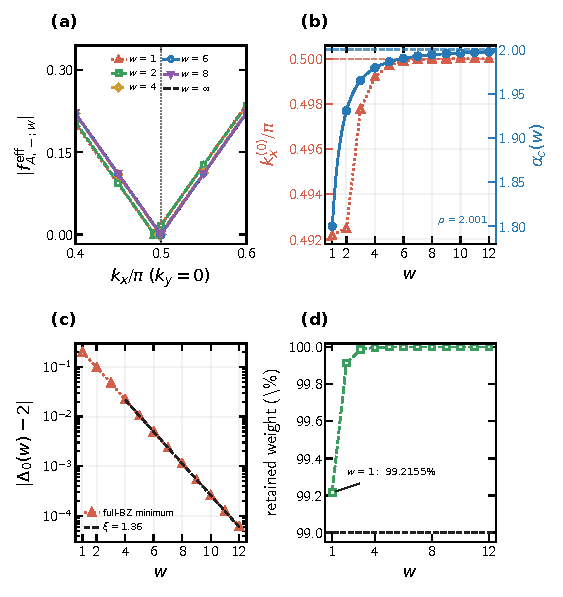
\includegraphics[width=\columnwidth]{ow_truncation_summary.pdf}
    \caption{Finite-envelope diagnostics for the fixed $\sigma^x$ trial pair in the convention of Eq.~\eqref{eq:spectral-vector-ci}. (a) BZ-normalized effective-form-factor amplitude of the lower-band $A$-family mode at $\alpha=1$ for $w=1,2,4,6,8$ and $w=\infty$, evaluated along $k_y=0$. Symbols mark the finite-$w$ zeros, and the vertical dotted line marks the unwindowed zero. (b) Position of the winding-$-1$ zero (red, left axis) and $\Gamma$-point gap-closing parameter $\alpha_c(w)$ of Eq.~\eqref{eq:TruncatedOWFrameHamiltonian} (blue, right axis). The blue solid curve is the fit in Eq.~\eqref{eq:TruncatedCriticalFit}; the dashed curves mark the corresponding $w=\infty$ limits. (c) Absolute error in the half-filling gap $\Delta_0(w)$ at $\alpha=1$. The red points are full-BZ minima, and the black dashed curve is the exponential tail fit for $w\geq4$. (d) Percentage of squared OW norm retained by the envelope; the dashed line marks $99\%$. The projector Fourier coefficients and zero/critical-point diagnostics use a $1024\times1024$ BZ quadrature, the gap search uses a $512\times512$ grid followed by continuous refinement, and the form-factor normalization uses a $241\times241$ grid. All curves are deterministic, and connecting lines are guides to the eye.}
    \label{fig:OWTruncationSummary}
\end{figure}

The extracted zero locations are shown on the red left axis of Fig.~\ref{fig:OWTruncationSummary}(b). The scalar-overlap zero exists throughout $0<\alpha<2$ and approaches the target-band gap-closing point at $\boldsymbol k=(0,0)$ as $\alpha\to2^-$ for every finite $w$. Therefore, the scalar overlap itself does not define a truncation-shifted Chern transition. To quantify the finite-$w$ spectrum and critical drift relevant to the truncated OW construction, we instead form the translation-invariant single-particle parent generated by the normalized OW frame built from the same fixed $\sigma^x$ trial pair,
\begin{align}
    h_w(\boldsymbol k)
    &=
    \sum_{\nu=A,B}
    \Bigl[
    \lvert\phi_{\nu,+;w}(\boldsymbol k)\rangle
    \langle\phi_{\nu,+;w}(\boldsymbol k)\rvert
    \nonumber\\[1pt]
    &\hspace{4.5em}
    -
    \lvert\phi_{\nu,-;w}(\boldsymbol k)\rangle
    \langle\phi_{\nu,-;w}(\boldsymbol k)\rvert
    \Bigr],
    \label{eq:TruncatedOWFrameHamiltonian}
\end{align}
where $\phi_{\nu,\pm;w}$ is the Bloch transform of the normalized truncated mode in Eq.~\eqref{eq:TruncatedOWWavefunction}, and $\nu=A,B$ labels the two $\sigma^x$ eigenvectors defined after Eq.~\eqref{eq:chi_CI}. At fixed $\alpha=1$, we define the half-filling gap by $\Delta_0(w)=\min_{\boldsymbol k,n}|E_n[h_w(\boldsymbol k)]|$. The parent is numerically traceless, so the direct occupied-to-empty band gap is $2\Delta_0(w)$. Figure~\ref{fig:OWTruncationSummary}(c) shows that $\Delta_0(w)$ rapidly approaches $\Delta_0(\infty)=2$. Although the onsite $w=0$ parent is gapped at $\alpha=1$, a gap alone does not imply a nonzero Chern number. At $w=0$, $\lvert\phi_{\nu,\pm;0}(\boldsymbol k)\rangle\propto P_{\pm,\boldsymbol r=0}\lvert\tau_\nu\rangle$ is independent of momentum, and hence so is $h_0(\boldsymbol k)$. Its occupied projector is therefore constant over the BZ, giving $\mc C_0=0$. Any winding zeros in its overlap with the original Chern band diagnose the obstruction of the target band, not an intrinsic topology of $h_0$. By contrast, at $w=1$ the parent remains well gapped, with $\Delta_0(1)=1.802426$, while the effective form factor retains its winding-$-1$ zero and more than $99\%$ of the OW weight. Thus, $w=1$ appears sufficient to keep the truncated parent gapped while retaining the relevant Chern-band overlap obstruction, and we use $w=1$ for the circuit analysis below. For $w\geq4$, the residual is accurately described by $|\Delta_0(w)-2|=0.410\exp(-w/1.358)$.

We next vary $\alpha$ to locate the transition of the truncated parent. The gap of $h_w$ closes at the $\Gamma$ point at a $w$-dependent value $\alpha_c(w)<2$, shown on the blue right axis of Fig.~\ref{fig:OWTruncationSummary}(b). For example, we find $\alpha_c(1)=1.800138$, $\alpha_c(2)=1.930755$, $\alpha_c(4)=1.979273$, $\alpha_c(8)=1.994307$, and $\alpha_c(12)=1.99739$. A fit over $w=3,\ldots,12$ to
\begin{equation}
    \alpha_c(w)
    =
    \alpha_\infty-\frac{A}{(w+b)^p}
    \label{eq:TruncatedCriticalFit}
\end{equation}
gives $\alpha_\infty=2.0000$, $A=0.405$, $b=0.415$, and $p=2.001$. Within the momentum-grid and fitting resolution, the finite-envelope drift therefore obeys
\begin{equation}
    2-\alpha_c(w)
    \simeq
    \frac{0.40}{(w+0.42)^2},
    \label{eq:TruncatedCriticalDrift}
\end{equation}
and extrapolates to the untruncated critical point $\alpha_c(\infty)=2$.

Finally, the fraction of squared OW norm retained inside the envelope, shown in Fig.~\ref{fig:OWTruncationSummary}(d), provides a separate measure of the truncation error. At $\alpha=1$, lattice and band symmetries make this retained fraction identical for all four choices of $\nu=A,B$ and $\pm$. We obtain $99.2155\%$, $99.9137\%$, $99.9979\%$, and $99.999997\%$ for $w=1,2,4,8$, respectively. In particular, even the smallest square envelope considered here, $w=1$, preserves more than $99\%$ of the squared wavefunction norm. The corresponding unsquared norm ratios are the square roots of these percentages.

\subsubsection{Unitary Feedback with Ancillas and Fermion Counting}
Following the construction of Bhuiyan et al.~\cite{BhuiyanPanJian2026}, we implement Gaussian unitary fSWAP feedback with anicallary fermion modes to correct undesired measurement outcomes. In the original design, a finite-sized bath of ancillas modes was tracked in addition to the dynamics of the physical modes. Given an undesired measurement outcome, the fSWAP gate corrects the occupation of the physical mode by swapping in a local ancilla mode. For a physical mode $\hat{\chi}^\dagger$ and ancilla mode $\hat{d}^\dagger$, the fSWAP gate is defined by
\begin{align}
    \fSWAP(\hat{\chi}^\dagger,\hat{d}^\dagger)
    &= \exp\left(\ii\frac{\pi}{2}(\hat{\chi}^\dagger-\hat{d}^\dagger)(\hat{\chi}-\hat{d})\right)\\
    &=
    \hat{\Id}-\hat{\mc{N}}-\hat{n}_a
    +\hat{\chi}^\dagger \hat{d}+\hat{d}^\dagger\hat{\chi}
    \label{eq:fSWAP}
\end{align}
where $\hat{\mc{N}}=\hat{\chi}^\dagger\hat{\chi}$ and $\hat{n}_a=\hat{d}^\dagger\hat{d}$ are the number operators for the physical and ancilla modes, respectively. 

However, the correction is inherently probablistic, as it depends on the ancilla mode having the desired occupancy. If the ancilla mode has the undesired occupancy, the fSWAP gate essentially becomes a do-nothing operation that fails to correct the occupancy of the physical mode. 

We can define an idealized `Markovian' version of the adaptive circuit construction of Ref.~\cite{BhuiyanPanJian2026} that does not require tracking a finite bath of ancilla modes. Rather, we can imagine that we have an infinite bath of ancilla modes and introduce a fresh ancilla with the desired outcome everytime a correction is needed in the physical system. This assumption enables deterministic feedback in the physical system, as we can always guarantee that the ancilla mode has the desired occupancy.

Concretely, an undesired outcome for the physical mode in the lower band $\hat{\Id}-\hat{\mathcal{N}}_{\bfr,\nu,-}$ can be corrected via fSWAP with a fresh ancilla mode $\hat{n}_{a}$ that is guaranteed to be occupied. Similarly, an undesired outcome for the physical mode in the upper band $\hat{\chi}_{\bfr,\nu,+}$ can be corrected via fSWAP with a fresh ancilla mode $\Id-\hat{n}_{\bfr,\nu,+}$ that is guaranteed to be empty. 

The ancilla modes can be traced out, leaving only operations that act on the physical modes. The resulting feedback operations consist of single fermion gain and loss
\begin{align}
    \braa{0}_a\fSWAP(\hat{\chi}_{\bfr,\nu,-}^\dagger,\hat{d}^\dagger)(\hat{\Id}-\hat{N}_{\bfr,\nu,-})\kett{1}_a &= \hat{\chi}_{\bfr,\nu,-}^\dagger\\
    \braa{1}_a\fSWAP(\hat{\chi}_{\bfr,\nu,+}^\dagger,\hat{d}^\dagger)\hat{\mc{N}}_{\bfr,\nu,+}\kett{0}_a &= \hat{\chi}_{\bfr,\nu,+}.
\end{align}
The upshot is that unitary feedback in the composite physical+ancilla system can be replaced by gain and loss operations in the physical system alone. Furthermore, note that the gain and loss operations remain Gaussian but no longer particle-number conserving. Rather, they are U(1)-equivariant, mapping the $q$-particle sector to the $q\pm1$-particle sector. At the level of quantum channel, the inclusion of gain and loss leads to a weak U(1) symmetry for the dynamics.

In recent literature, these gain and loss operations are often referred to as \emph{fermion counting} operations. We see here that fermion counting operations can be implemented via unitary operations with ancilla in larger Hilbert space.

\subsubsection{Adaptive Circuit Model}
The circuit model consists of two types of measurement-feedback layers, one that fills the lower-band OW modes and one that empties the upper-band OW modes. Each elementary time step consists of a projective measurement of the occupation of one normalized truncated OW mode, followed by a gain or loss operation only when the outcome disagrees with its target occupation. 

To simplify notation, we introduce the composite index $i=(\bfr, \nu)\in\mathbb{Z}^2\times\{A,B\}$ to label the unit-cell center $\bfr$ and trial spinor $\nu$. The \emph{truncated} lower-band OW mode is denoted by $\hat{\chi}_{i,-}$, and the truncated upper-band OW mode is $\hat{\chi}_{i,+}$. The corresponding number operators are $\hat{\mathcal N}_{i,-}=\hat{\chi}_{i,-}^\dagger\hat{\chi}_{i,-}$ and $\hat{\mathcal N}_{i,+}=\hat{\chi}_{i,+}^\dagger\hat{\chi}_{i,+}$.


Let $\{\xi_{t,i,\pm}\}$ be a collection of Bernoulli random variables that records the measured occupation of $\hat{\chi}_{i,\pm}$ at elementary circuit time step $t=1,\dots,T$. Thus, $\xi_{t,i,\pm}=0$ denotes an empty mode and $\xi_{t,i,\pm}=1$ denotes an occupied mode. The Bernoulli random variable is distributed according to the Born rule
\begin{equation}
    \xi_{t,i,\pm}\in\{0,1\}\sim\mr{Ber}(\langle\hat{\mathcal N}_{i,\pm}\rangle_{t}),
\end{equation}
where $\langle\hat{\mathcal N}_{i,\pm}\rangle_{t}=\Tr[\hat{\mathcal N}_{i,\pm}\hat\rho_{t}]$ is the expectation value of the number operator in the normalized, record-conditioned state $\hat\rho_{t}$ immediately before the measurement. In other words, $\xi_{t,i,\pm}=1$ with probability $\langle\hat{\mathcal N}_{i,\pm}\rangle_{t}$ and $\xi_{t,i,\pm}=0$ with probability $1-\langle\hat{\mathcal N}_{i,\pm}\rangle_{t}$.

With this notation, the operator-valued random variable or \emph{Kraus operator} for lower-band ($-$) measurement+feedback at time step $t$ is
\begin{align}
    \hat{K}_{t,i,-}(\xi_{t,i,-}) = \xi_{t,i,-}\hat{\mathcal N}_{i,-} + (1-\xi_{t,i,-})\hat{\chi}_{i,-}^\dagger
\end{align}
whereas for the upper band ($+$) we have
\begin{align}
    \hat{K}_{t,i,+}(\xi_{t,i,+}) = (1-\xi_{t,i,+})\left(\hat{\Id}-\hat{\mathcal N}_{i,+}\right) + \xi_{t,i,+}\hat{\chi}_{i,+}.
\end{align}
It is easy to verify that these Kraus operators are Gaussian and satisfy the POVM condition
\begin{equation}
    \sum_{\xi=0,1}\hat K_{t,i,\pm}^{\dagger}(\xi)\hat K_{t,i,\pm}(\xi)=\hat{\Id}.
\end{equation}
However, the trajectory-averaged evolution is \emph{not} Gaussian.

At each unit-cell center $\bfr$, we apply the updates in the order $(A,+)$, $(A,-)$, $(B,+)$, and $(B,-)$, and a complete circuit cycle sweeps through every center. Because truncated OW modes centered on nearby unit cells overlap, the corresponding occupation measurements generally do not commute. For the trajectory-resolved results and the channel comparison in Sec.~\ref{sec:TrajectoryAveragedDynamics}, we fix the schedule $\mc S$ to the canonical \texttt{raster\_y} order, increasing $y$ at fixed $x$ before advancing to the next $x$ column. Ordering is part of the protocol and is not averaged implicitly.

To make this ordering explicit, let $\Lambda=\mathbb Z_{N_x}\times\mathbb Z_{N_y}$ denote the set of unit-cell centers on a finite periodic lattice, with $|\Lambda|=N_{\mr{uc}}=N_xN_y$. At elementary time step $t$, the composite index and band label satisfy
\begin{equation}
    i_t=(\bfr_t,\nu_t)\in\Lambda\times\{A,B\},
    \qquad \sigma_t\in\{-,+\}.
\end{equation}
One complete cycle contains
\begin{equation}
    T=4N_{\mr{uc}}
\end{equation}
elementary measurement-feedback operations. The factor of four arises because both trial spinors $\nu=A,B$ are measured in both bands $\sigma=\pm$ at every unit-cell center. For a realized record $\boldsymbol\xi=(\xi_1,\ldots,\xi_T)$, where $\xi_t\equiv\xi_{t,i_t,\sigma_t}$, the corresponding cycle-wise Kraus operator is
\begin{align}
    \hat{\mc{K}}^{\mr{cyc}}_{\boldsymbol\xi}
    &=\prod_{t=1}^{T}
    \hat K_{t,i_t,\sigma_t}(\xi_t)\nonumber\\
    &\equiv\hat K_{T,i_T,\sigma_T}(\xi_T)\cdots
    \hat K_{2,i_2,\sigma_2}(\xi_2)
    \hat K_{1,i_1,\sigma_1}(\xi_1),
    \label{eq:AdaptiveCycleKraus}
\end{align}
where the explicit second line fixes our convention that the $t=1$ operation acts first. The probability and normalized state associated with this record are, respectively,
\begin{align}
    p(\boldsymbol\xi)
    &=\Tr\!\left[\hat{\mc{K}}^{\mr{cyc}}_{\boldsymbol\xi}\hat\rho_0
    \hat{\mc{K}}_{\boldsymbol\xi}^{\mr{cyc}\dagger}\right],
    \label{eq:AdaptiveRecordProbability}\\
    \hat\rho_{\boldsymbol\xi}
    &=\frac{\hat{\mc{K}}^{\mr{cyc}}_{\boldsymbol\xi}\hat\rho_0
    \hat{\mc{K}}_{\boldsymbol\xi}^{\mr{cyc}\dagger}}
    {p(\boldsymbol\xi)}.
    \label{eq:AdaptiveConditionalState}
\end{align}
The physical state ensemble is therefore the Born-weighted collection $\{p(\boldsymbol\xi),\hat\rho_{\boldsymbol\xi}\}$.

The domain-wall geometry and the elementary measurement-feedback step are summarized in Fig.~\ref{fig:DomainWallAdaptiveCircuit}.

\begin{widetext}
    \begin{center}
        \centering
        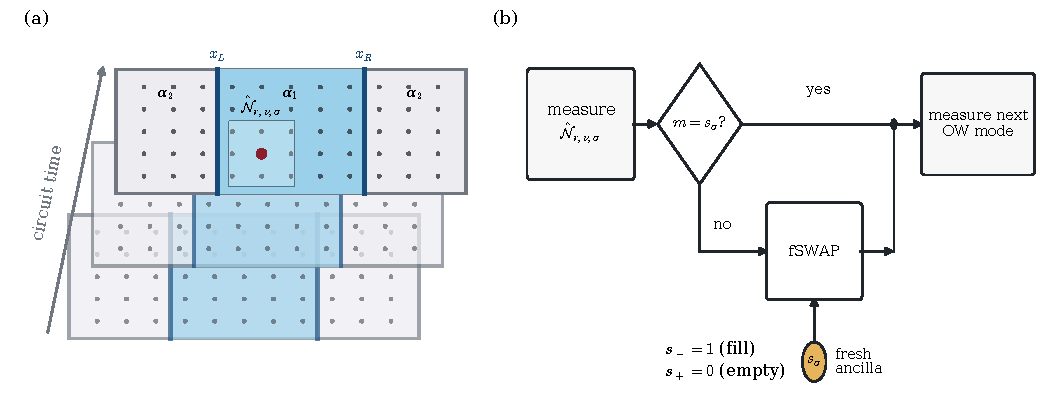
\includegraphics[width=\textwidth]{domain_wall_adaptive_circuit.pdf}
        \begin{minipage}{0.96\textwidth}
            \captionof{figure}{\textbf{Domain-wall adaptive circuit.} (a) The $N_x\times N_y$ domain-wall geometry, with periodic boundary conditions in both directions, is repeated through circuit time. The two interfaces are marked in deep blue, and a local OW occupation operator is indicated within its $3\times3$ unit-cell support. (b) The OW occupation is measured with a Born-random outcome $m$. If $m\neq s_\sigma$, an fSWAP with a fresh ancilla restores the target occupation. The two branches then join before the next OW mode is measured.}
            \label{fig:DomainWallAdaptiveCircuit}
        \end{minipage}
    \end{center}
\end{widetext}

\subsubsection{Gaussian Dynamics and Real-Space Chern Number}
Because every measurement and correction step is Gaussian, it is most convenient to follow the dynamics through the two-point function
\begin{equation}
    C_{ij}=\operatorname{Tr}\!\left(\hat\rho\,\hat c_i^\dagger\hat c_j\right),
    \qquad
    G=2C-\mathbf{1}.
    \label{eq:ComplexCovarianceDefinition}
\end{equation}
Here $G$ is the centered complex covariance. Its eigenvalues lie in $[-1,1]$, and a pure number-conserving Gaussian trajectory obeys $C^2=C$, or equivalently $G^2=\mathbf{1}$.

For a normalized truncated OW wavefunction $W_j$, where $j=(\bf{r},\nu, \pm)$, we define the single-particle projector in the index ordering used by the simulator as
\begin{equation}
    P_j=(W_jW_j^\dagger)^{\mathsf T},
    \qquad
    Q_j=\mathbf{1}-P_j
    \label{eq:StoredOWProjector}
\end{equation}
where $W_j\in\mathbb{C}^{2N_x N_y}$ is represented as a column vector over local orbital and unit cell indices.
Writing $m\in\{0,1\}$ for the measured occupation, $s\in\{0,1\}$ for its target value, and $\eta_m=2m-1$, $\eta_s=2s-1$, the exact conditional update is~\cite{BhuiyanPanJian2026}
\begin{equation}
    G'_{m,s}
    =Q_j\left(\mathbf{1}+\eta_mGP_j\right)^{-1}GQ_j
    +\eta_sP_j .
    \label{eq:ConditionalComplexCovarianceUpdate}
\end{equation}
Using the projector in Eq.~\eqref{eq:StoredOWProjector}, the Born probability for the measured occupation is
\begin{equation}
    p_j(m\mid G)
    =\frac{1+\eta_m\operatorname{Tr}(P_jG)}{2}.
    \label{eq:OWBornProbability}
\end{equation}
The circuit schedule first selects $j=(\bfr,\nu,\sigma)$. We then draw $m=1$ with probability $W_j^{\mathsf T}CW_j^*$ and $m=0$ with probability $1-W_j^{\mathsf T}CW_j^*$. The target occupation is not sampled: it is fixed by the band label, with $s_-=1$ for a lower-band mode and $s_+=0$ for an upper-band mode. Thus, $G$ determines the Born distribution, the random draw determines $m$, and the prescribed band label determines $s$. Feedback is applied only when $m\neq s_\sigma$.

The inverse in Eq.~\eqref{eq:ConditionalComplexCovarianceUpdate} is only a rank-one resolvent and is nonsingular on every outcome with nonzero Born probability. Each conditioned trajectory therefore remains Gaussian and is completely specified by $G$. The correction resets the measured OW mode to its target occupation. The Born-weighted trajectory average, however, is generally not itself a Gaussian state.

To evaluate topology, we first restore the spectral-projector ordering,
\begin{equation}
    \Gamma=C^{\mathsf T}
    =\left(\frac{\mathbf{1}+G}{2}\right)^{\mathsf T}.
    \label{eq:SpectralProjectorOrdering}
\end{equation}
The transpose in Eq.~\eqref{eq:SpectralProjectorOrdering} simply converts between the stored two-point-function ordering and the usual one-body projector ordering. Following Appendix~C.3 of Kitaev~\cite{Kitaev2006}, we choose a disk of radius $R$ centered at a general trijunction $\boldsymbol r_0$ and divide it into three counterclockwise sectors $A$, $B$, and $C$, as shown in Fig.~\ref{fig:RealSpaceChernPartition}. Both orbitals at a given unit cell are assigned to the same sector. The disk radius must be much larger than the correlation length of the system, $R\gg\xi_{\mr{corr}}$, while remaining inside the homogeneous bulk region. If $\Gamma_{XY}$ denotes the block with rows in $X$ and columns in $Y$, the real-space Chern number used here is
\begin{equation}
  \begin{aligned}
    \mc C_G(\boldsymbol r_0,R)
    =12\pi\operatorname{Re}\!\Big\{\ii\big[\,
    &\operatorname{tr}(\Gamma_{CA}\Gamma_{AB}\Gamma_{BC})\\[-2pt]
    &-\operatorname{tr}(\Gamma_{AC}\Gamma_{CB}\Gamma_{BA})
    \,\big]\Big\}.
    \end{aligned}
    \label{eq:KitaevRealSpaceChern}
\end{equation}
In the numerics, we evaluate the same expression directly from the occupied frame $V$ using
\begin{equation}
    \Gamma=(VV^\dagger)^{\mathsf T}=V^*V^{\mathsf T},
    \label{eq:OccupiedFrameProjectorTranspose}
\end{equation}
which avoids constructing the full covariance matrix. 
\begin{figure}[t]
    \centering
    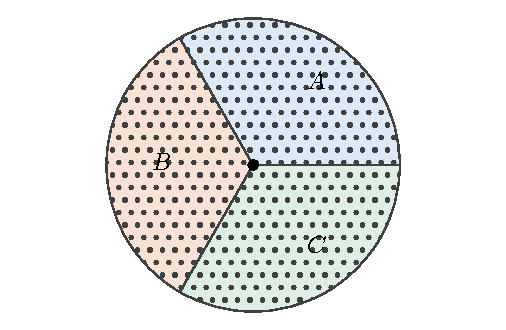
\includegraphics[width=\columnwidth]{real_space_chern_partition.pdf}
    \caption{\textbf{Real-space Chern partition.} A disk of radius $R$, centered at $\boldsymbol r_0$, is divided into three counterclockwise sectors $A,B,C$. Both orbitals of a unit cell are assigned to the same sector.}
    \label{fig:RealSpaceChernPartition}
\end{figure}

\subsubsection{Domain-Wall Free Bulk Validation}
We first check that the idealized dynamics prepares the intended bulk state without introducing a domain wall. Here we use square systems with $N_x=N_y=L$. We initialize random pure states at half filling and evolve them for 40 cycles at $\alpha=1$ with perfect correction. Figure~\ref{fig:UniformBulkChernDynamics} shows that the sample-averaged real-space Chern number rapidly approaches $\mc C_G=1$ for every system size and OW truncation considered. The convergence is noticeably faster than in BPJ~\cite{BhuiyanPanJian2026}. In the idealized model used here, a fresh ancilla with the required occupation is always available, so every undesired measurement outcome is corrected. In BPJ, the finite ancillary bath corrects an undesired outcome only with finite probability. The measurement outcomes remain Born stochastic; only the feedback following an undesired outcome is deterministic. 

To separate this finite-size dependence from the initial transient, we discard the first 20 cycles and form a late-time estimate from cycles 21--40. For each pair $(L,n_{\rm shell})$, we pool these 20 late-time values over the $S=100$ trajectories, giving a $100\times20$ sample-cycle ensemble. Figure~\ref{fig:UniformBulkChernFiniteSize} shows the resulting mean and its standard error. This late-time averaging suppresses the residual cycle-to-cycle fluctuations about the stationary plateau and gives a more stable estimate than the value from a single terminal cycle. We see that the deviation of the real-space Chern number from unity typically decreases with system size for every choice of $n_{\rm shell}$. This provides evidence that our adaptive circuit prepares the intended bulk topological state with truncated OW modes in the thermodynamic limit.

\begin{center}
    \centering
    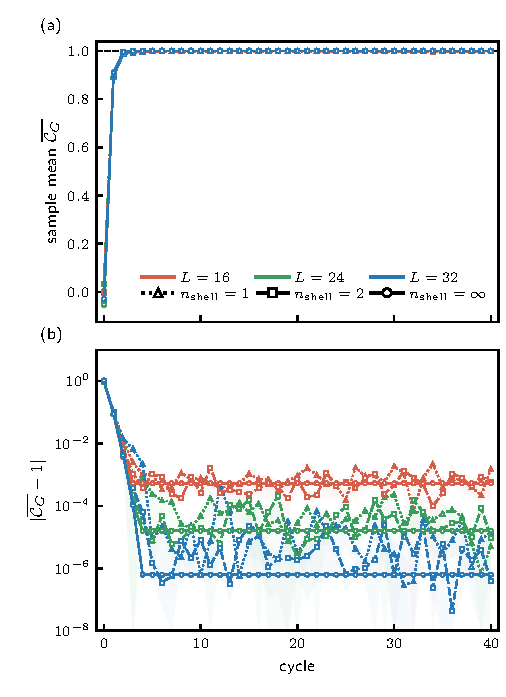
\includegraphics[width=\columnwidth]{bulk_chern_cycle_convergence.pdf}
    \begin{minipage}{0.96\columnwidth}
        \captionof{figure}{\textbf{Domain-wall-free bulk preparation.} (a) Sample-averaged real-space Chern number $\overline{\mc C_G}$ and (b) $|\overline{\mc C_G}-1|$. Red, green, and blue denote $L=16,24,32$, while markers and line styles denote $n_{\rm shell}=1,2,\infty$. We use $\boldsymbol r_0=(L/2,L/2)$ and $R=0.4L$. Shading is the standard error over $S=100$ independent trajectories.}
        \label{fig:UniformBulkChernDynamics}
    \end{minipage}
\end{center}

\begin{center}
    \centering
    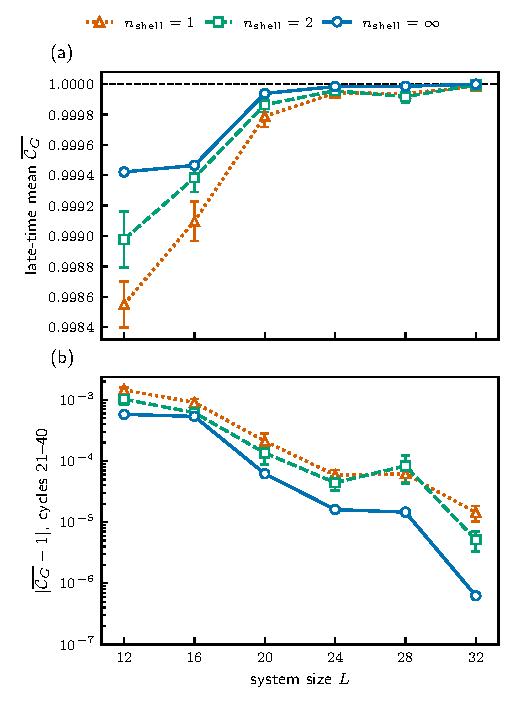
\includegraphics[width=\columnwidth]{bulk_chern_final_size_scaling.pdf}
    \begin{minipage}{0.96\columnwidth}
        \captionof{figure}{\textbf{Late-time finite-size convergence.} (a) Mean real-space Chern number and (b) its absolute deviation from unity over the $100\times20$ sample-cycle ensemble formed from cycles 21--40, using the same central partition as Fig.~\ref{fig:UniformBulkChernDynamics}. Error bars are the standard error over the 2,000 sample-cycle values; lines are guides to the eye.}
        \label{fig:UniformBulkChernFiniteSize}
    \end{minipage}
\end{center}

The gain and loss corrections can change the total particle number along an individual record, so we also check how far the ensemble wanders from half filling. We define
\begin{equation}
    \Delta Q_\xi(t)=Q_\xi(t)-L^2,
    \qquad
    f_\xi(t)=\frac{Q_\xi(t)}{2L^2}.
    \label{eq:GlobalChargeDeviation}
\end{equation}
Every conditioned pure Gaussian trajectory has a definite integer value of $Q_\xi(t)$. The fluctuations in Fig.~\ref{fig:UniformBulkChargeFluctuations} are therefore record-to-record fluctuations of the total charge, rather than an intrinsic quantum variance within one trajectory. For finite OW truncation, the relative charge spread remains small and generally decreases with system size. The dense construction remains exactly at half filling throughout the evolution.

\begin{center}
    \centering
    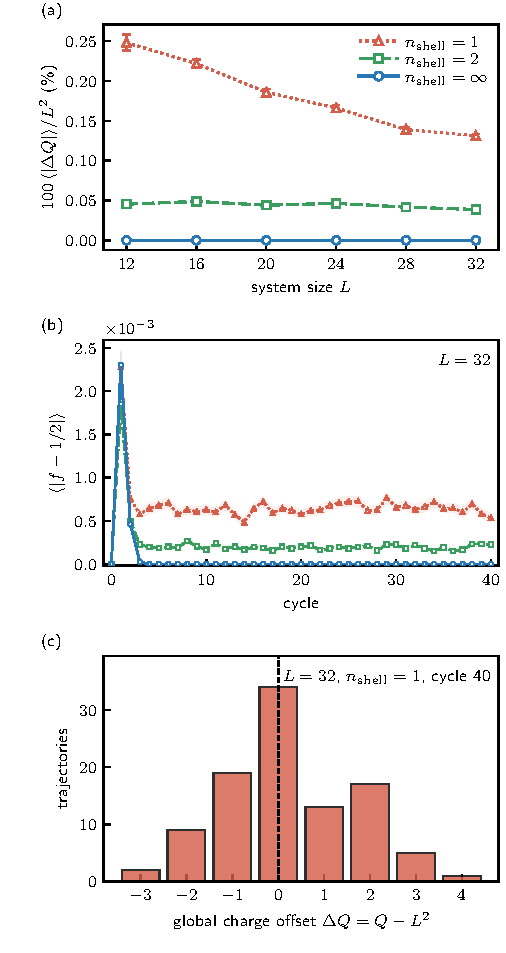
\includegraphics[width=\columnwidth]{bulk_global_charge_fluctuations.pdf}
    \begin{minipage}{0.96\columnwidth}
        \captionof{figure}{\textbf{Global charge about half filling.} (a) Late-time mean absolute relative deviation from half filling for cycles 21--40. (b) Mean absolute filling-fraction deviation at $L=32$. (c) Cycle-40 distribution of $\Delta Q=Q-L^2$ for $L=32$ and $n_{\rm shell}=1$. Late-time averages are first formed within each trajectory; error bars and bands are the standard error over $S=100$ independent trajectories.}
        \label{fig:UniformBulkChargeFluctuations}
    \end{minipage}
\end{center}
\clearpage

\subsection{Dynamical Domain Walls in Adaptive Circuits}
\subsubsection{Domain Wall Geometry and Hard vs Soft Walls}
We introduce a domain wall by making the Chern-insulator parameter depend on the unit-cell center of the OW mode. Let the topological slab occupy $x_L\leq x<x_R$. We define
\begin{equation}
    \alpha_{\bfr}=
    \begin{cases}
        \alpha_1, & x_L\leq x<x_R,\\
        \alpha_2, & \text{otherwise},
    \end{cases}
    \label{eq:UnitCellDependentAlpha}
\end{equation}
where $\alpha_1$ controls the slab and $\alpha_2$ controls the exterior. Henceforth, we fix $\alpha_2=30$, deep in the trivial phase, and vary only $\alpha_1$. The OW mode centered at $\bfr$ is constructed from the uniform projector with parameter $\alpha_{\bfr}$. Since the system is periodic in $x$, one topological slab necessarily produces two interfaces with opposite orientations. The slab is chosen to have size $N_x/2$ in the $x$ direction, so that the two interfaces are separated by $N_x/2$ unit cells. The slab is centered at $x=0$, so that the left interface is at $x_L=-N_x/4$ and the right interface is at $x_R=N_x/4$. Nevertheless, periodic boundary conditions are still imposed in both directions.

We have empirically determined two ways to implement a domain wall in the adaptive circuit. For the `soft' wall, we keep the full finite-range support of every OW mode. Modes centered on opposite sides of the interface can therefore overlap.

For the hard wall, we additionally remove the part of each OW mode that crosses the interface and then renormalize the remaining wavefunction. The controller support therefore terminates at the edge of the topological slab, as shown in Fig.~\ref{fig:SoftHardDomainWalls}. In this sense, the hard wall acts much like open boundary conditions for the adaptive circuit: OW measurements on one side do not extend into the other side. It is not literally an open-boundary Hamiltonian, since the full lattice remains periodic and the exterior degrees of freedom are still present.

\begin{center}
    \centering
    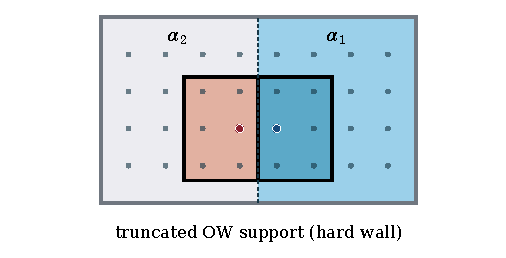
\includegraphics[width=\columnwidth]{ow_overlap_truncation_schematic.pdf}
    \begin{minipage}{0.96\columnwidth}
        \captionof{figure}{\textbf{Hard domain-wall support.} The lattice sites immediately adjacent to the interface center two OW modes on opposite sides. Each nominal support is truncated at the interface and renormalized, so no measured OW mode crosses between the $\alpha_2$ and $\alpha_1$ regions.}
        \label{fig:SoftHardDomainWalls}
    \end{minipage}
\end{center}

\subsubsection{Endpoint Entanglement and Charge Fluctuations}
We first study the hard wall at the topological point $\alpha_1=1$, with
$\alpha_2=30$ outside the slab.  The calculation uses $N_x=20$,
$N_y=30,35,40,45,50,55,60$, and $S=100$ independent Born trajectories at
each circumference.  Every trajectory starts from an independently sampled
pure state, uses $n_{\rm shell}=1$, the raster-$y$ update order, and perfect
correction, and is evolved in complex128 arithmetic to the endpoint
$t=2N_y$.  This subsection concerns that endpoint ensemble only.  In
particular, it is not pooled with the earlier cycle-resolved entropy data.

For a periodic strip beginning at $y_0$ and extending through $A_y$ cells,
we take
\begin{equation}
 A(y_0,A_y)=[0,N_x)\times[y_0,y_0+A_y)\pmod{N_y}.
 \label{eq:HardWallStripRegion}
\end{equation}
If $R_{A,\xi}$ denotes the rows of the occupied frame restricted to this
strip, its restricted two-point function and occupation spectrum are
\begin{equation}
 G_{A,\xi}=R_{A,\xi}R_{A,\xi}^{\dagger}
 =U_{A,\xi}\operatorname{diag}(\nu_{a,\xi})U_{A,\xi}^{\dagger}.
 \label{eq:HardWallRestrictedCorrelation}
\end{equation}
This form lets us evaluate the subsystem observables without materializing
the full-system covariance matrix.  The von Neumann and R\'enyi entropies are
\begin{align}
 S_{1,\xi}(y_0,A_y)
 &=-\sum_a\left[\nu_a\log\nu_a+(1-\nu_a)\log(1-\nu_a)\right],
 \nonumber\\
 S_{q,\xi}(y_0,A_y)
 &=\frac{1}{1-q}\sum_a\log\!\left[\nu_a^q+(1-\nu_a)^q\right].
 \label{eq:HardWallRenyiEntropies}
\end{align}
Here and below, $q=2,3$ for the R\'enyi entropies.
The same spectrum gives the intrinsic subsystem charge variance
\begin{equation}
 F_{A,\xi}(y_0,A_y)
 =\operatorname{tr}\!\left[G_{A,\xi}(\mathbf{1}_A-G_{A,\xi})\right]
 =\sum_a\nu_a(1-\nu_a).
 \label{eq:HardWallChargeVariance}
\end{equation}
This is the fluctuation of the subsystem charge inside one conditioned state.
It is not the record-to-record variance of the mean charge.  Entanglement and
charge fluctuations are closely related for free fermions because both are
spectral functions of the same restricted correlation matrix~\cite{KlichLevitov2009,SongFlindtRachel2011}.
The subscript $A$ labels the subsystem; throughout this subsection, $q$ is
reserved exclusively for the R\'enyi index.

The infrared interpretation is a pair of spatially separated chiral
$1+1$d conformal field theories, one on each wall.  In the replica
construction, $\operatorname{Tr}\hat\rho_{A,\xi}^q$ is a two-point function
of branch-point twist fields.  A conformal map from the plane to a cylinder
of circumference $N_y$ replaces the interval length by the chord distance
and fixes the logarithmic coefficient.  For one chiral branch the twist
field has dimension $h_q=(c_w/24)(q-1/q)$, so that its contribution is
$(c_w/12)(1+1/q)X(A_y)$~\cite{CalabreseCardy2004}.  The full-$x$ strip cuts
both walls.  Their positive entanglement contributions add even though the
walls propagate in opposite directions.  For two symmetry-related walls,
the total slope is therefore $m_q=(c_w/6)(1+1/q)$, and the $c_q$ extracted
below measures the central-charge magnitude of either wall.

The charge fit probes different CFT data.  The long-wavelength density is
the time component of a $U(1)$ current whose modes obey
$[J_m,J_n]=k_w m\,\delta_{m+n,0}$.  The integer $k_w$ is the Kac--Moody
level: once the microscopic unit of charge is fixed, it normalizes the
current--current correlator.  A charge-one chiral complex fermion has
$k_w=1$~\cite{DiFrancescoMathieuSenechal1997}.  Integrating the cylinder
correlator over an interval gives a one-wall variance
$(k_w/2\pi^2)X(A_y)$ plus a nonuniversal constant.  The two walls again add,
because a variance is insensitive to their opposite propagation directions,
so the measured full-strip slope is $m_F=k_w/\pi^2$.  Thus the entropy and
charge fits test the central charge and the $U(1)$ current level
independently; a single chiral complex-fermion branch predicts
$c_w=k_w=1$.

Within each trajectory, we average both $S_{q,\xi}(y_0,A_y)$ and
$F_{A,\xi}(y_0,A_y)$ uniformly over all $N_y$ translated origins.  We denote
the resulting curves by $\overline S_{q,\xi}(A_y)$ and
$\overline F_{A,\xi}(A_y)$.  The translated origins are therefore not counted
as independent samples.  At fixed $N_y$, our statistical objects are the
ensemble-mean curves
\begin{align}
 \left\langle\overline S_q(A_y)\right\rangle_\xi
 &=\frac{1}{S}\sum_{\xi=1}^S\overline S_{q,\xi}(A_y),
 \nonumber\\
 \left\langle\overline F_A(A_y)\right\rangle_\xi
 &=\frac{1}{S}\sum_{\xi=1}^S\overline F_{A,\xi}(A_y).
 \label{eq:HardWallMeanCurves}
\end{align}
We first form these averages over the $S=100$ independent trajectories and
only then fit the window $A_y=8,\ldots,\lfloor N_y/2\rfloor$ against
\begin{equation}
 X(A_y)=\log\!\left[\frac{N_y}{\pi}
 \sin\!\left(\frac{\pi A_y}{N_y}\right)\right].
 \label{eq:HardWallLogChord}
\end{equation}
The Calabrese--Cardy prediction for the two interfaces intersected by the
strip is~\cite{CalabreseCardy2004}
\begin{align}
 \left\langle\overline S_q(A_y)\right\rangle_\xi
 &=m_qX(A_y)+b_q,
 &c_q&=\frac{6q}{q+1}m_q,
 \nonumber\\
 \left\langle\overline F_A(A_y)\right\rangle_\xi
 &=m_FX(A_y)+b_F,
 &k&=\pi^2m_F.
 \label{eq:HardWallCftFits}
\end{align}
The fit is performed on the mean curve, but its uncertainty is still the
ordinary sampling uncertainty of the trajectory ensemble.  If $\mathbf a$ is
the fixed unweighted-OLS projection that maps a vector of strip values to its
slope, $\overline{\mathbf y}$ is the ensemble-mean curve, and
$\boldsymbol\Sigma_{\mathbf y}$ is the sample covariance of the complete
trajectory curves across strip widths, then
\begin{equation}
 m=\mathbf a^{\mathsf T}\overline{\mathbf y},\qquad
 \operatorname{SEM}(m)^2=
 \mathbf a^{\mathsf T}\frac{\boldsymbol\Sigma_{\mathbf y}}{S}\mathbf a.
 \label{eq:HardWallMeanCurveSem}
\end{equation}
This retains all within-trajectory covariance between different $A_y$ values;
the strip widths are not treated as independent observations.  No bootstrap
resampling and no fit-residual uncertainty are used.  Because every
trajectory at a given size has the same $X$ grid and unweighted linear fit,
the central value obtained by fitting the mean curve is algebraically equal
to the mean of the individually fitted slopes.  We verify that identity
numerically, but Eq.~\eqref{eq:HardWallCftFits}---average first, fit
second---defines the estimator used below.

At $N_y=60$, fits to the four ensemble-mean curves give
\begin{align}
 c_1&=1.0402(39), & c_2&=1.0383(40),
 \nonumber\\
 c_3&=1.0378(39),
 \label{eq:HardWallEndpointCentralCharges}
\end{align}
where the parenthetical digits are covariance-propagated trajectory SEMs.
The three R\'enyi estimates track one another throughout the size series.
Their common few-percent upward offset and the nonmonotonic point at $N_y=55$
are retained as finite-size information rather than removed by an
extrapolation.

The chord coordinate also permits a direct collapse test across circumference.
For each circumference, let $A_N^\star=\lfloor N_y/2\rfloor$.  We subtract
that trajectory's measured half-strip value before averaging, so the plotted
coordinates are
\begin{align*}
 \left\langle\Delta\overline S_{q,N,i}\right\rangle_\xi
 &=\left\langle
 \overline S_{q,\xi}(A_{y,i})-
 \overline S_{q,\xi}(A_N^\star)
 \right\rangle_\xi,\\
 \Delta x_{N,i}
 &=X_N(A_{y,i})-X_N(A_N^\star),\\
 &=\log\!\left[
 \frac{\sin(\pi A_{y,i}/N_y)}
      {\sin(\pi A_N^\star/N_y)}\right].
\end{align*}
Every mean curve is therefore anchored exactly at the origin, including the
odd circumferences.  We fit one line through that fixed origin over
$A_{y,i}=8,\ldots,A_N^\star$.  With $w_N=1/n_N$, the fitted slope is
\begin{align*}
 m_q^{\mathrm{anch}}
 &=\frac{\displaystyle\sum_N w_N\sum_i
 \Delta x_{N,i}\left\langle\Delta\overline S_{q,N,i}\right\rangle_\xi}
 {\displaystyle\sum_N w_N\sum_i(\Delta x_{N,i})^2},\\
 c_q^{\mathrm{anch}}&=\frac{6q}{q+1}m_q^{\mathrm{anch}}.
\end{align*}
The factor $w_N=1/n_N$ assigns equal total weight to every circumference,
rather than allowing the larger systems to dominate simply because they
provide more $A_y$ values.  We quote the through-origin coefficient
$R_0^2=1-\mathrm{RSS}/\sum_{N,i}w_N
\langle\Delta\overline S_{q,N,i}\rangle_\xi^2$, because the origin is
fixed by the measured half-strip value rather than estimated by regression.
The slope SEM is propagated from the full covariance of the anchored
trajectory curves, independently for each size, through the same weighted
linear projection.

Figure~\ref{fig:HardWallEndpointEntropy} gives
$c_1^{\mathrm{anch}}=1.04295\pm0.00183$,
$c_2^{\mathrm{anch}}=1.04083\pm0.00189$, and
$c_3^{\mathrm{anch}}=1.04030\pm0.00189$.  The corresponding $R_0^2$ values are
$0.999923$, $0.999936$, and $0.999938$.  These are joint fits to the seven
ensemble-mean curves, not representative-trajectory fits.

\begin{figure}[!htbp]
    \centering
    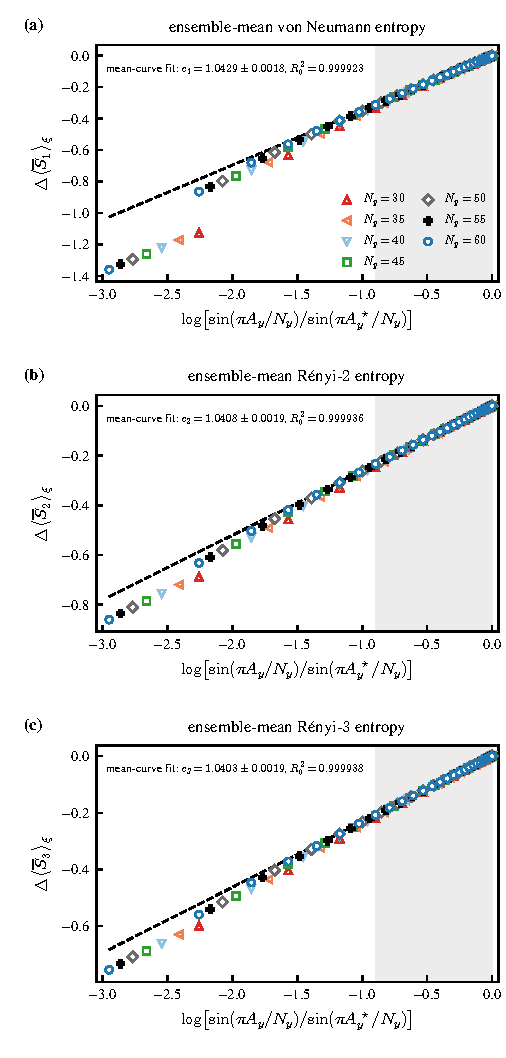
\includegraphics[width=0.96\columnwidth]{endpoint_entropy_mean_curve_size_collapse_3x1.pdf}
    \caption{\textbf{Ensemble-mean endpoint entropy collapse.}
    Hard-wall data at $N_x=20$, $t=2N_y$, and $S=100$ independent trajectories
    per circumference.  Panels show (a) von Neumann, (b) R\'enyi-2, and
    (c) R\'enyi-3 entropy.  Periodic origins are averaged within each
    trajectory; trajectories are then averaged before fitting.  Each mean
    curve is anchored by
    $\Delta\langle\overline S_q\rangle_\xi=
    \langle\overline S_q(A_y)-\overline S_q(A_N^\star)\rangle_\xi$ and
    $\Delta X=\log[\sin(\pi A_y/N_y)/\sin(\pi A_N^\star/N_y)]$.
    Bars are pointwise trajectory SEMs and can be smaller than the open
    markers.  The gray band marks $A_y=8,\ldots,A_N^\star$; the black dashed
    line is one equal-size-weighted through-origin fit.  Quoted coefficient
    errors propagate the full trajectory covariance across strip widths.}
    \label{fig:HardWallEndpointEntropy}
\end{figure}

The charge sector gives the same answer without reusing the entropy formula.
At $N_y=60$, the fit to the ensemble-mean variance curve gives
\begin{equation}
 k=1.0389(40).
 \label{eq:HardWallEndpointLevel}
\end{equation}
The corresponding entropy--charge ratios are formed from coefficients of the
paired ensemble-mean curves,
\begin{align}
 \frac{c_1}{k}&=1.00123(33), &
 \frac{c_2}{k}&=0.99944(14),
 \nonumber\\
 \frac{c_3}{k}&=0.99894(27).
 \label{eq:HardWallEntropyChargeRatios}
\end{align}
Their ordinary SEMs use the joint trajectory covariance of the entropy and
charge slope projections, followed by standard ratio propagation.  Thus most
of the finite-size shift is common to the two estimators: their relative
normalization agrees at the $10^{-3}$ level even though either coefficient
separately remains a few percent above one.

For the direct charge collapse, we apply the same endpoint anchor before the
trajectory average,
\begin{equation}
 \left\langle\Delta\overline F_{A,N,i}\right\rangle_\xi
 =\left\langle\overline F_{A,\xi}(A_{y,i})
 -\overline F_{A,\xi}(A_N^\star)\right\rangle_\xi.
 \label{eq:HardWallChargeAnchor}
\end{equation}
The equal-size-weighted through-origin fit gives
$m_F^{\mathrm{anch}}=0.105518(191)$, hence
$k^{\mathrm{anch}}=1.04142\pm0.00189$, with $R_0^2=0.999933$.
Figure~\ref{fig:HardWallEndpointCharge} shows the seven ensemble means on the
same charge-sector line.

\begin{figure}[!htbp]
    \centering
    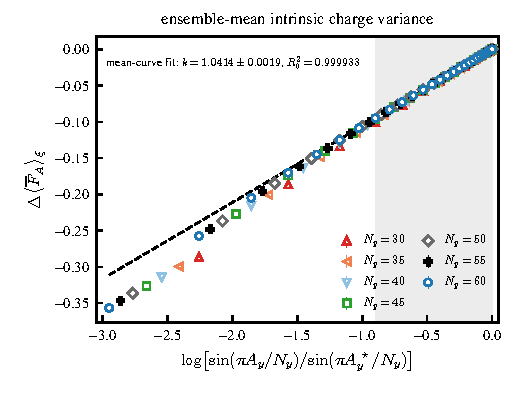
\includegraphics[width=0.96\columnwidth]{endpoint_charge_variance_mean_curve_size_collapse_1x1.pdf}
    \caption{\textbf{Ensemble-mean endpoint charge-variance collapse.}
    Intrinsic subsystem charge variance at $N_x=20$, $t=2N_y$, and $S=100$.
    Origins are averaged within a trajectory, each trajectory is anchored at
    $A_N^\star=\lfloor N_y/2\rfloor$, and the anchored curves are then averaged.
    Bars are pointwise trajectory SEMs and can be smaller than the open
    markers.  The gray band marks $A_y=8,\ldots,A_N^\star$; the black dashed
    line is one equal-size-weighted through-origin fit.  Its uncertainty
    propagates the full trajectory covariance across strip widths.}
    \label{fig:HardWallEndpointCharge}
\end{figure}

The size-resolved mean-curve fits are collected in
Fig.~\ref{fig:HardWallEndpointMeanCurveScaling}.  At every $N_y$, each of the
100 trajectory curves are averaged first, and the resulting mean curve is
then fitted using Eq.~\eqref{eq:HardWallCftFits}.  The bars are the
full-covariance trajectory SEMs from Eq.~\eqref{eq:HardWallMeanCurveSem}, not
regression-residual errors.  Dashed segments simply connect adjacent sizes and
are not finite-size fits.

\begin{figure}[!htbp]
    \centering
    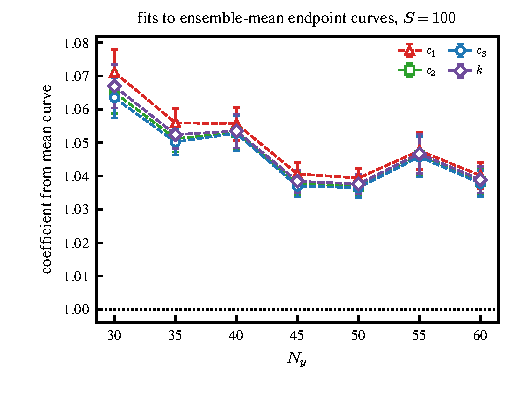
\includegraphics[width=0.96\columnwidth]{endpoint_mean_curve_cq_k_scaling_1x1.pdf}
    \caption{\textbf{Endpoint coefficients from ensemble-mean curves.}
    At each circumference, $c_1,c_2,c_3$, and $k$ are extracted after first
    averaging the 100 trajectory-resolved strip curves.  Bars are ordinary
    trajectory sampling SEMs propagated with the full covariance across
    $A_y$.  Dashed lines join adjacent sizes as guides to the eye; the dotted
    line marks the free-fermion value $c=k=1$.}
    \label{fig:HardWallEndpointMeanCurveScaling}
\end{figure}

\begin{samepage}
Finally, Fig.~\ref{fig:HardWallEndpointContours} displays the spatial
decomposition for the fixed half strip $A(0,N_y/2)$ after cellwise averaging
over the $S=100$ independent trajectories.  Let $h_q(x)$ denote the scalar entropy kernel in
Eq.~\eqref{eq:HardWallRenyiEntropies}, promoted spectrally to the matrix
function $h_q(G_{A,\xi})$.  The cell-resolved contours are simply its
diagonal density and the corresponding diagonal density of the charge
variance,
\begin{align}
 s_{q,\xi}(\boldsymbol r;A)
 &=\sum_\mu\langle\boldsymbol r,\mu\rvert
 h_q(G_{A,\xi})\lvert\boldsymbol r,\mu\rangle,
 \nonumber\\
 f_{A,\xi}(\boldsymbol r)
 &=\sum_\mu\langle\boldsymbol r,\mu\rvert G_{A,\xi}
 (\mathbf{1}_A-G_{A,\xi})\lvert\boldsymbol r,\mu\rangle.
 \label{eq:HardWallSpatialContours}
\end{align}
\end{samepage}
They satisfy the exact closure relations
\begin{align}
 \sum_{\boldsymbol r\in A}s_{q,\xi}(\boldsymbol r;A)
 =\operatorname{tr}h_q(G_{A,\xi})=S_{q,\xi}(A),
 \nonumber\\
 \sum_{\boldsymbol r\in A}f_{A,\xi}(\boldsymbol r)
 =\operatorname{tr}[G_{A,\xi}(\mathbf{1}_A-G_{A,\xi})]=F_{A,\xi}.
 \label{eq:HardWallContourClosure}
\end{align}
These maps are not origin averaged: they resolve the particular region
$[0,20)\times[0,30)$, with the two hard walls at $x=5$ and $x=15$.
The contour is constructed within each trajectory and then averaged cellwise
over the $S=100$ independent trajectories.
The measured closure error is below $9\times10^{-15}$.  The maps include the
nonuniversal short-distance boundary contribution and are therefore used to
show where the endpoint observable resides, not to extract $c$ or $k$ by
themselves.

\begin{figure}[!htbp]
    \centering
    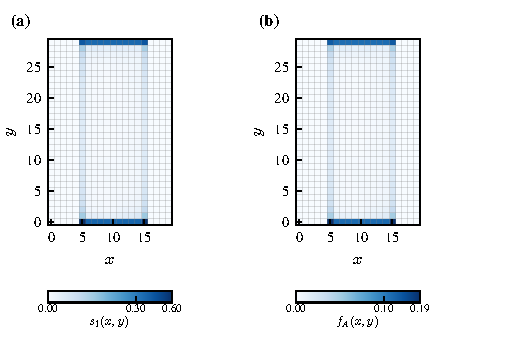
\includegraphics[width=\columnwidth]{endpoint_entropy_charge_contours_1x2.pdf}
    \caption{\textbf{Fixed-half-strip contours.}
    (a) Von Neumann entropy and (b) intrinsic charge-variance contours for
    $[0,20)\times[0,30)$ at $N_y=60$ and $t=2N_y$, averaged cellwise over
    $S=100$ independent trajectories.  Gray gridlines resolve individual unit
    cells; wall positions are not overlaid.  Each panel uses an independent
    square-root-normalized Blues scale from zero to its maximum.}
    \label{fig:HardWallEndpointContours}
\end{figure}

Taken together, the endpoint data support a hard-wall state with the entropy
and $U(1)$ charge content of a level-one complex-fermion boundary theory.  The
agreement among the independently fitted ensemble-mean $q=1,2,3$ entropy
curves and the ensemble-mean charge-variance curve is stronger than a single
von Neumann fit.  It does not by itself establish chirality, and it does not
yet establish that the soft-wall construction has the same finite-size
behavior.

\subsubsection{Chiral Central Charge}
The nontrivial statement is not only that the two-wall strip has the entropy
coefficient of a $c=1$ theory.  It is that this coefficient separates in real
space into one-half from each wall.  In the conventional nonchiral
Cardy--Calabrese normalization, $S=(c/3)X+\cdots$.  A static interval in a
possibly chiral boundary theory instead measures
$(c_L+c_R)X/6$~\cite{CalabreseCardy2004,CastroDetournayIqbalPerlmutter2014}.
Thus one complex chiral mode contributes a slope $1/6$, exactly half of the
usual $c=1$ coefficient $1/3$.  The full-$x$ strip intersects both interfaces
and only reveals their sum.  The all-$A_y$ entropy-contour ensemble resolves
that sum in the transverse direction.  For each trajectory, the contour is
first aligned in $\delta y=(y-y_0)\bmod N_y$ and averaged over every periodic
origin $y_0$.  We then define the predeclared three-column wall integrals
\begin{align}
 \overline S^{\mathrm{wall}}_{L,\xi}(A_y)
 &=\sum_{x=4}^{6}\sum_{\delta y=0}^{A_y-1}
   \overline s_{\xi,A_y}(x,\delta y),
 \nonumber\\
 \overline S^{\mathrm{wall}}_{R,\xi}(A_y)
 &=\sum_{x=14}^{16}\sum_{\delta y=0}^{A_y-1}
   \overline s_{\xi,A_y}(x,\delta y).
 \label{eq:WallResolvedContourEntropy}
\end{align}
The two windows are centered on the hard walls at $x=5$ and $x=15$.
They retain the localized boundary contribution without assigning the entire
left or right half of the slab to a wall.

For a purely chiral wall, $c_L+c_R$ equals the magnitude of the chiral central
charge.  It is useful to display the same slope in both normalizations:
\begin{align}
 m_w&=\frac{c_L^{(w)}+c_R^{(w)}}{6}
 =\frac{|c_-^{(w)}|}{6},
 \nonumber\\
 3m_w&=\frac{|c_-^{(w)}|}{2},
 \qquad c_-^{(w)}\equiv c_R^{(w)}-c_L^{(w)}.
 \label{eq:WallChiralCentralChargeSlope}
\end{align}
Accordingly, $3m_w=1/2$ is the expected entropy weight of one unit-chiral
wall when measured in the usual full-strip normalization.  Entropy determines
$|c_-^{(w)}|$, but not its sign.  The sign must be supplied by a directional
probe, such as the flux-threading analysis below.  This distinction matters
because the two interfaces have opposite orientations: their signed chiral
central charges cancel even though their positive entropy weights add.  This
separation between the static entropy magnitude and the anomalous directional
response is the same distinction emphasized in the chiral-entanglement and
domain-wall anomaly-inflow literature~\cite{IqbalWall2016,HughesLeighParrikarRamamurthy2016}.

We use an independent contour-resolved ensemble with $N_x=20$,
$N_y=30,35,40,45,55$, and $S=100$ trajectories at each circumference.
Within each trajectory, each wall curve is anchored at
$A_N^\star=\lfloor N_y/2\rfloor$ before the trajectory average.  We then fit
one through-origin slope over $A_y=8,\ldots,A_N^\star$, with equal total
weight assigned to each circumference, exactly as in
Fig.~\ref{fig:HardWallEndpointEntropy}.  Ordinary trajectory SEMs are
propagated using the full covariance across $A_y$.

The two wall-resolved fits give the half-unit entropy weights
\begin{align}
 3m_L&=0.51865(133), & |c_-^{(L)}|&=6m_L=1.0373(27),
 \nonumber\\
 3m_R&=0.48722(160), & |c_-^{(R)}|&=6m_R=0.9744(32).
 \label{eq:WallResolvedChiralCentralCharges}
\end{align}
Their sum is
\begin{equation}
 3(m_L+m_R)=1.00587(197),
 \label{eq:WallAveragedChiralCentralCharge}
\end{equation}
only $0.59\%$ above the expected $1/2+1/2=1$.  The quoted error retains
the left--right covariance within each trajectory.  The residual difference
between the two three-column windows is a transverse-localization effect:
changing the window redistributes contour weight between the wall and its
tails.  We therefore interpret the resolved half-unit contributions and their
paired sum as the clean statement, rather than interpreting $m_L-m_R$ as two
different boundary theories.  This spatial decomposition is information that
the full-strip entropy fit cannot provide by itself.

\begin{figure}[!htbp]
    \centering
    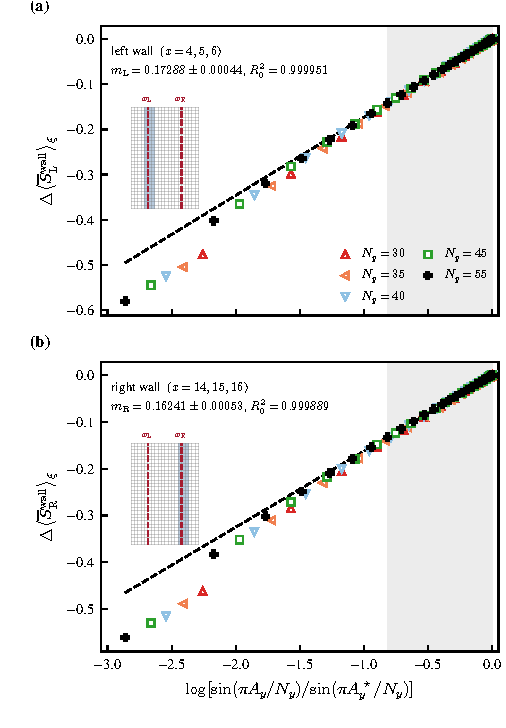
\includegraphics[width=0.96\columnwidth]{hard_wall_chiral_central_charge_2x1.pdf}
    \caption{\textbf{Half-unit entropy coefficient from each chiral wall.}
    Independent hard-wall contour data at $N_x=20$, $t=2N_y$, and
    $N_y=30,35,40,45,55$.  Panels integrate the origin-averaged von Neumann
    contour over (a) $x=\{4,5,6\}$ and (b) $x=\{14,15,16\}$.  Each trajectory
    is anchored at $A_N^\star=\lfloor N_y/2\rfloor$ before the trajectory
    average.  Bars are ordinary trajectory SEMs and can be smaller than the
    open markers.  Gray marks the fit window
    $A_y=8,\ldots,A_N^\star$; the black dashed line is one
    equal-size-weighted through-origin fit.  Insets use a representative
    $20\times30$ unit-cell grid to mark both domain walls and shade the
    three-column contour window used in the corresponding panel.  In the
    ordinary full-strip normalization, the weights are $3m_L=0.51865(133)$
    and $3m_R=0.48722(160)$, whose paired sum is $1.00587(197)$, consistent
    with $1/2+1/2$.  Equivalently, $6m_{L/R}=|c_-^{(L/R)}|$; entropy alone
    does not determine their opposite signs.}
    \label{fig:HardWallChiralCentralCharge}
\end{figure}

As a deterministic control, we apply the same entropy estimators to the
half-filled ground state of the static flattened OW parent
\begin{equation}
 H_{\mathrm{OW}}
 =\sum_R\left(P_{A+}(R)+P_{B+}(R)-P_{A-}(R)-P_{B-}(R)\right).
 \label{eq:HardWallFlattenedOWParent}
\end{equation}
The projectors in Eq.~\eqref{eq:HardWallFlattenedOWParent} use the identical
hard-wall, $n_{\rm shell}=1$, $\alpha_1=1$, and $\alpha_2=30$ construction as
the monitored circuit. At each $N_y$, we diagonalize the conserved-$k_y$
blocks and occupy the lowest $N_xN_y$ one-body levels. We then repeat the
same half-strip anchoring, fit window, equal-size weighting, and three-column
wall integrations used above. Translation invariance along $y$ makes a
single contour in relative coordinates the exact periodic-origin average for
this reference state.

Figure~\ref{fig:HardWallFlattenedEntropyBenchmark} shows the size-resolved
comparison. The flattened parent gives a joint full-strip value
$c_1=0.99935$ and equal wall weights
$3m_L=3m_R=0.49929$. By comparison, the monitored endpoint ensemble gives
$c_1=1.04295(183)$, $3m_L=0.51865(133)$, and
$3m_R=0.48722(160)$. The separate fits also expose the finite-size trend.
For the flattened reference, even $N_y$ is essentially exact, while the
odd-size full-strip error falls from $0.368\%$ at $N_y=35$ to $0.153\%$ at
$45$ and $0.082\%$ at $55$. In the monitored ensemble, the full-strip excess
drops from $6.97\%$ at $N_y=30$ to roughly $3.7\%$ at the largest sizes. The
paired wall-weight excess improves more sharply, from $2.08\%$ at $N_y=30$
to $0.10\%$ at $45$ and $0.13\%$ at $55$, even though neither individual
wall is monotone. The deterministic left--right equality rules out a
geometric bias between the two predeclared windows. More importantly, these
coefficients are finite-size estimators, not one-sided bounds: even the
flattened reference lies slightly below the asymptotic half-unit value. The
monitored left and right deviations occur with opposite signs, while their
paired sum, $3(m_L+m_R)=1.00587(197)$, stays close to one. We therefore read
the residual asymmetry as finite-time contour weight shifting between each
three-column window and its tails, rather than as different wall theories.

\begin{figure}[!htbp]
    \centering
    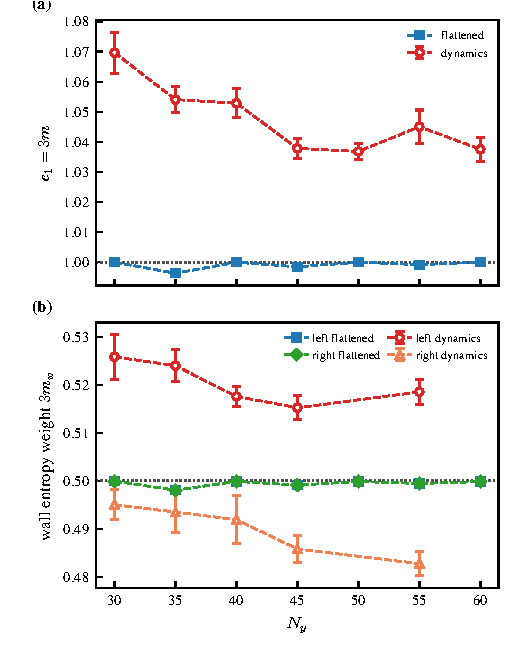
\includegraphics[width=0.96\columnwidth]{hard_wall_dynamics_vs_flattened_entropy_coefficients_2x1.pdf}
    \caption{\textbf{Monitored endpoints against the flattened-parent benchmark.}
    (a) Full-strip von Neumann coefficient $c_1=3m$ and (b) three-column
    wall weights $3m_w$ versus circumference. Open red/orange markers are
    obtained by averaging the monitored trajectory curves first and then
    fitting; bars are ordinary trajectory SEMs propagated with the full
    covariance across $A_y$. Filled blue/green markers are deterministic
    half-filled ground-state results for
    Eq.~\eqref{eq:HardWallFlattenedOWParent} and have no sampling error.
    Dotted lines mark $c_1=1$ and $3m_w=1/2$. The wall-resolved monitored
    campaign contains $N_y=30,35,40,45,55$; the flattened control is shown at
    all seven available circumferences.}
    \label{fig:HardWallFlattenedEntropyBenchmark}
\end{figure}

\subsubsection{Boundary and Bulk Correlation Scaling}
We next resolve the correlations along the wall without first averaging over
the transverse direction.  For a single trajectory $\xi$, define
\begin{align}
 C_{G,\xi}(x,r_y)
 &=\frac{1}{2N_y}\sum_{y,\mu,\nu}
 \left|C^{(\xi)}_{(x,y,\mu),(x,y+r_y,\nu)}\right|^2,
 \nonumber\\
 C_{G,\xi}^{\mathrm{av}}(r_y)
 &=\frac{1}{N_x}\sum_{x=0}^{N_x-1}C_{G,\xi}(x,r_y).
 \label{eq:EndpointSquaredCorrelator}
\end{align}
Here $C^{(\xi)}_{ij}=\operatorname{Tr}(\hat\rho_\xi\hat c_i^\dagger\hat c_j)$,
the $y$ coordinate is periodic, and both orbital indices are summed.  The
overline below denotes an arithmetic average over the independent
trajectories, after forming the squared correlator.  Thus we do not square
the averaged two-point function or average its logarithm.

This positive squared correlator has a direct density interpretation.
Write $\hat n_i=\hat c_i^\dagger\hat c_i$ and
$\langle\delta\hat n_i\delta\hat n_j\rangle_\xi
=\langle\hat n_i\hat n_j\rangle_\xi
-\langle\hat n_i\rangle_\xi\langle\hat n_j\rangle_\xi$.
Wick's theorem for a charge-conserving Gaussian trajectory gives
\begin{equation}
 \langle\delta\hat n_i\delta\hat n_j\rangle_\xi
 =\delta_{ij}C^{(\xi)}_{ii}-|C^{(\xi)}_{ij}|^2.
 \label{eq:EndpointDensityWickIdentity}
\end{equation}
For distinct modes, the connected density correlator is therefore the
negative of the squared two-point function.  With the total cell density
$\hat n_{x,y}=\sum_\mu\hat n_{x,y,\mu}$, the precise normalization of
our observable is
\begin{align}
 C_{G,\xi}(x,r_y)=-\frac{1}{2N_y}\sum_y
 \langle\delta\hat n_{x,y}\delta\hat n_{x,y+r_y}\rangle_\xi,
 \nonumber\\[-2pt]
 r_y\not\equiv0\pmod{N_y}.
 \label{eq:EndpointCellDensityCorrelator}
\end{align}
The factor $1/2$ is our per-orbital normalization.  At coincident cells the
contact term in Eq.~\eqref{eq:EndpointDensityWickIdentity} must be retained.
The connected subtraction is made inside each trajectory before the
ensemble average.  Forming a connected correlator of the mixed ensemble
instead adds the classical trajectory covariance of the local mean
densities, which is not included in the plotted quantity.

For a free chiral fermion, the fermion field has scaling dimension $1/2$,
so its two-point function decays as $d_{N_y}^{-1}$ and the squared
correlator has the critical prediction
\begin{equation}
 \overline{C_G^{\mathrm{av}}(r_y)}\sim A\,d_{N_y}(r_y)^{-\beta},
 \qquad \beta_{\mathrm{crit}}=2,
 \label{eq:EndpointCorrelatorCriticalPrediction}
\end{equation}
provided the long-distance signal is boundary dominated.  The chord is
$d_{N_y}(r_y)=(N_y/\pi)\sin(\pi r_y/N_y)$.  Figure~\ref{fig:HardWallCorrelatorSummary}
shows the distinction directly: at $\alpha_1=1$ the long-distance signal
survives the average over $x$, whereas at $\alpha_1=3$ it drops rapidly.
At $N_y=60$, the exact wall columns carry the largest long-distance
correlations.  The neighboring columns and the slab center have much
smaller amplitudes.  For this dataset we use the saved array coordinates
$x=0,\ldots,19$, with $x_L=5$ and $x_R=15$.

For the size collapse, we remove each circumference's amplitude using its
measured antipodal value.  With $r_\star=N_y/2$, set
\begin{align}
 X_N(r_y)&=\log\frac{d_{N_y}(r_y)}{d_{N_y}(r_\star)},
 \nonumber\\
 Y_N(r_y)&=\log\frac{\overline{C_G^{\mathrm{av}}(r_y)}}
                         {\overline{C_G^{\mathrm{av}}(r_\star)}}.
 \label{eq:EndpointCorrelatorCollapse}
\end{align}
Both coordinates vanish at the measured anchor; no fitted vertical shift
is introduced.  We fit $Y_N=-\beta X_N$ on
$8\leq r_y\leq N_y/2$, assigning equal total weight to each
circumference.  Explicitly, if $\mathcal W_N$ contains the $n_N$ selected
separations,
\begin{equation}
 \beta=-\frac{\sum_N n_N^{-1}\sum_{r_y\in\mathcal W_N}X_NY_N}
                  {\sum_N n_N^{-1}\sum_{r_y\in\mathcal W_N}X_N^2}.
 \label{eq:EndpointCorrelatorJointFit}
\end{equation}
The six-size fit gives $\beta=2.1903$, without constraining the power to
two.  We use $r_y\geq8$ to separate this fit from the short-distance
transient, while retaining the full independent interval through $N_y/2$.
The selected windows contain 5, 7, 9, 13, 18, and 23 separation values for
the six circumferences; $N_y=60$ does not supply 60 independent distances.
Moving the lower endpoint to five gives $\beta=2.2016$.
The earlier $2,\ldots,\lfloor N_y/4\rfloor$ window gave $2.2291$;
extending that same lower cutoff to $N_y/2$ gave $2.2282$.
Thus the lower cutoff, rather than the upper one, accounts for most of
the shift.  The antipodal normalization is the same in all these checks.
The collapse supports an
algebraic boundary contribution, but these finite-size effective exponents
remain above the ideal prediction.  This varies the circumference at
fixed $N_x=20$, not both dimensions of the system.  The fit is to logarithms
of ensemble-mean curves, not an average of sample-wise exponents.

\begin{figure}[!htbp]
 \centering
 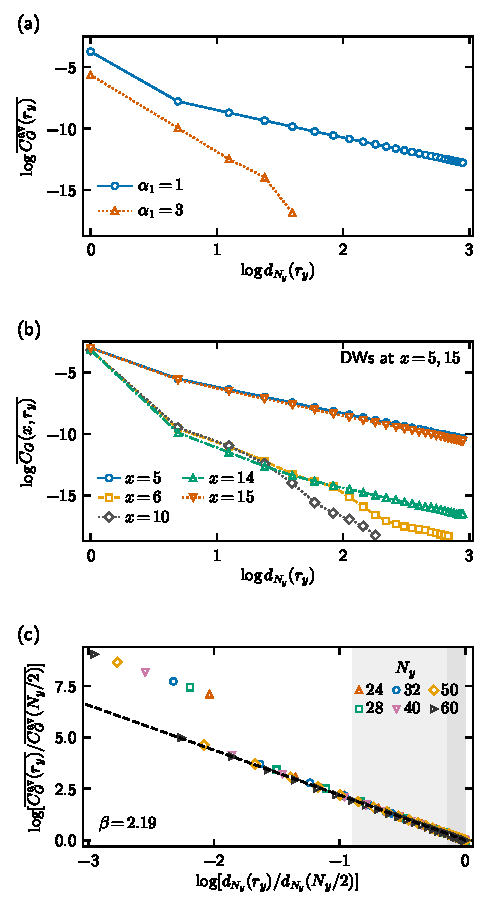
\includegraphics[width=\columnwidth]{hard_wall_correlator_summary_3x1.pdf}
 \caption{\textbf{Endpoint correlation scaling.}
 Hard walls, $N_x=20$, $\alpha_2=30$, $n_{\rm shell}=1$, $t=2N_y$;
 $S=100$ independent pure half-filled initial states per ensemble,
 Born-conditioned exterior preparation, raster-$y$ perfect correction,
 and complex128 arithmetic.
 (a) Full-$x$ average at $N_y=60$, comparing $\alpha_1=1$ and $3$.
 (b) $\alpha_1=1$, $N_y=60$: walls $x=5,15$, adjacent cells $x=6,14$,
 and slab center $x=10$.
 (c) Antipodally normalized collapse of the $\alpha_1=1$ means for
 $N_y=24,28,32,40,50,60$.  The black dashed line is the equal-size-weighted
 fit $Y_N=-\beta X_N$ on $8\leq r_y\leq N_y/2$, giving $\beta=2.1903$.
 Light gray covers the union of the size-specific fit ranges; darker gray
 marks their common interval.  Each size retains its color and open symbol
 at every separation, including points outside its fit window.
 The dashed continuation outside the fit ranges is an extrapolation.
 All means precede logarithms; no uncertainty bands are shown.
 Only $1\leq r_y\leq N_y/2$ is used.  The $10^{-8}$ cutoff in (a,b)
 is for display, not a certified numerical floor; it excludes no fitted
 points in (c).  Colored lines in (a,b) guide the eye.}
 \label{fig:HardWallCorrelatorSummary}
\end{figure}

The boundary and bulk contributions need not be disentangled by subtracting
entropies.  For this particular observable, the spatial bookkeeping is
exactly additive.  Partition the columns into
$B=\{5,6,14,15\}$ and its complement $U$.  Let $\overline C_B$ and
$\overline C_U$ be the correlators averaged within their respective
sets and over trajectories.  Then
\begin{equation}
 \overline{C_G^{\mathrm{av}}}
 =\frac{|B|}{N_x}\overline C_B
 +\frac{|U|}{N_x}\overline C_U.
 \label{eq:EndpointCorrelatorSpatialSum}
\end{equation}
No independence assumption is needed: Eq.~\eqref{eq:EndpointSquaredCorrelator}
only samples pairs at the same $x$.  Correlations between different columns
would belong to a different observable.  The complement $U$ includes the
slab interior and exterior, and is not assumed to be a pure bulk sector.
For $N_y=60$, the four selected boundary columns contribute $99.35\%$ of
the full-$x$ average at $r_y=5$ and $99.95\%$ at $r_y=30$.

If the regional curves can be approximated by algebraic and exponential
pieces, this sum has the form
\begin{equation}
 \overline{C_G^{\mathrm{av}}(r_y)}
 \simeq A_{\mathrm e}d_{N_y}(r_y)^{-\beta}
 +A_{\mathrm b}\left[e^{-r_y/\xi_C}+e^{-(N_y-r_y)/\xi_C}\right].
 \label{eq:EndpointCorrelatorMixedDecay}
\end{equation}
The coefficients include the spatial weights.  This is a phenomenological
description of the squared correlators, not an exact decomposition of the
single-particle amplitudes: splitting $C=C_{\mathrm e}+C_{\mathrm b}$
inside one matrix element would generate an interference term in $|C|^2$.
At $x=10$, the observed short-distance curve is well described by
$\log\overline{C_G(10,r_y)}=b-r_y/\xi_C$ on $r_y=2,\ldots,6$, with
$\xi_C=0.6552$ unit cells.  This is the decay length of the squared
correlator over that window, not a claim of purely exponential behavior
at every separation.  A small algebraic tail can coexist in the interior
at finite slab width.  Once the exponential contribution has decayed,
the positive boundary contribution controls the full-$x$ average even
though only a few columns carry most of its weight.


\subsubsection{Antipodal Bipartite Mutual Information}
As a separate endpoint observable, we take a full-$x$ strip $a$ of width
$w=N_y/4$ beginning at $y_0$ and an equal strip $b$ shifted by $N_y/2$ around
the periodic $y$ direction, as shown in the inset of
Fig.~\ref{fig:HardWallBipartiteMutualInformation}.  Both orbitals are included.
For each trajectory, we first form the nonlinear combination
\begin{equation}
 I_{a,b;\xi}(y_0)=S_\xi(a)+S_\xi(b)-S_\xi(a\cup b),
 \label{eq:HardWallTrajectoryMutualInformation}
\end{equation}
then average it over the $N_y/2$ distinct translations and finally over the
$S$ independent trajectories.

The dashed reference in Fig.~\ref{fig:HardWallBipartiteMutualInformation}
follows from the exact disconnected-interval entropy of a massless free Dirac
field.  On the line, for interval lengths $\ell_a$ and $\ell_b$ separated by a
gap $d$, cancellation of the cutoff and local boundary terms gives the
following result, with all logarithms taken to be natural:
\begin{align}
 I_{a,b}
 &=\frac{c}{3}\log\!\left[
   \frac{(\ell_a+d)(\ell_b+d)}{d(\ell_a+\ell_b+d)}\right]
 =-\frac{c}{3}\log(1-x),\nonumber\\
 x&=\frac{\ell_a\ell_b}{(\ell_a+d)(\ell_b+d)}.
 \label{eq:HardWallFreeDiracLineMI}
\end{align}
This factorized expression is special to the free Dirac theory
\cite{CasiniHuerta2009}; a generic CFT two-interval entropy contains an
additional theory-dependent twist-field scaling function
\cite{CalabreseCardyTonni2009}.

Mapping to a circle replaces every endpoint separation $s$ by the chord
$D(s)=(N_y/\pi)\sin(\pi s/N_y)$.  The common factors cancel in the cross-ratio,
so for the geometry in the inset of
Fig.~\ref{fig:HardWallBipartiteMutualInformation}, where
$\ell_a=\ell_b=w$ and $d=N_y/2-w$,
\begin{align}
 x&=\frac{D(\ell_a)D(\ell_b)}
 {D(\ell_a+d)D(\ell_b+d)}\nonumber\\
 &=\sin^2\!\left(\frac{\pi w}{N_y}\right),\nonumber\\
 I_{a,b}^{\mathrm{Dirac}}
 &=-\frac{c}{3}\log\!\left[
 \cos^2\!\left(\frac{\pi w}{N_y}\right)\right].
 \label{eq:HardWallFreeDiracCircleMI}
\end{align}
The two counterpropagating domain-wall branches supply the left- and
right-moving sectors of one $c=1$ Dirac theory.  Therefore $w=N_y/4$ fixes
$x=1/2$ at every size and yields the benchmark value
\begin{equation}
 I_{a,b}^{\mathrm{Dirac}}=\frac{\log 2}{3}=0.2310491\ldots .
 \label{eq:HardWallQuarterStripMI}
\end{equation}
This is a fixed-cross-ratio limit: all interval lengths and gaps grow in the
same proportion, so critical scale invariance predicts a nonzero constant,
not a logarithmic divergence.  A logarithm would instead arise if the strip
width grew while the physical gap remained fixed, driving $x\to1$.

Figure~\ref{fig:HardWallBipartiteMutualInformation} shows the completed
hard-wall $n_{\rm shell}=1$ trajectory ensemble.  At $\alpha_1=1$ the mean
decreases from $0.2602$ at $N_y=20$ to $0.2466$ at $N_y=28$, approaching the
Dirac reference from above.  The larger peak near $\alpha_1=1.7$ also decreases
with size; it is a finite-size, finite-time crossover containing bulk as well
as wall correlations, rather than a distinct saturation value or a stable
$c>1$ wall theory.

\begin{figure}[!htbp]
    \centering
    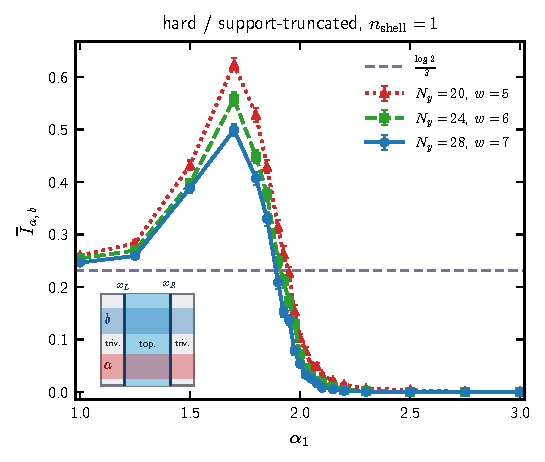
\includegraphics[width=\columnwidth]{hard_wall_nshell1_bmi_with_geometry.pdf}
    \caption{\textbf{Hard-wall antipodal mutual information.}
    Sample- and origin-averaged $\overline I_{a,b}$ for $N_x=20$,
    $N_y=20,24,28$, $w=N_y/4$, $n_{\rm shell}=1$, and $\alpha_2=30$.
    The inset shows the opposite full-$x$ strips $a$ and $b$ and the domain
    walls at $x_L$ and $x_R$.
    Each point contains $S=100$ independent random pure half-filled Born
    trajectories evolved with perfect correction and raster-$y$ ordering to
    the endpoint $t=2N_y$; $I_{a,b}$ is formed for each trajectory and origin
    before either average.  Error bars are one sample-wise standard error.
    The horizontal dashed line is the parameter-free free-Dirac prediction
    $(\log 2)/3$ from Eq.~\eqref{eq:HardWallQuarterStripMI}, not a fit.  The
    sweep was executed from $\alpha_1=3$ to $1$, while the displayed axis uses
    increasing order.}
    \label{fig:HardWallBipartiteMutualInformation}
\end{figure}

\subsubsection{Spectral Chirality from Flux Threading}
\label{sec:HardWallSpectralChirality}

The endpoint entropy and charge fluctuations establish the expected
one-dimensional boundary content, but these quantities do not determine its
direction of propagation.  We therefore probe chirality by threading flux
through the periodic $y$ direction of each trajectory-resolved endpoint
projector.  This is a spectral-flow calculation performed after the monitored
circuit has ended.  It does not rerun the measurement record and it is not a
real-time current measurement.

For trajectory $\xi$, let $P_{\xi,0}=\Gamma_{\xi,0}$ be the endpoint
projector in the spectral ordering of Eq.~\eqref{eq:SpectralProjectorOrdering}.
We form the flattened parent
\begin{equation}
 H_{\xi}(0)=\mathbf{1}-2P_{\xi,0}
 \label{eq:EndpointFlattenedParent}
\end{equation}
and thread a transverse flux by
\begin{align}
 [\widetilde H_{\xi}(\phi)]_{rs}
 &=[H_{\xi}(0)]_{rs}
 \exp\!\left[\ii\phi\frac{d_y(r,s)}{N_y}\right],\nonumber\\
 H_{\xi}(\phi)
 &=\frac{1}{2}\left[\widetilde H_{\xi}(\phi)
 +\widetilde H_{\xi}^{\dagger}(\phi)\right],
 \label{eq:EndpointUniformFluxThreading}
\end{align}
where $d_y(r,s)$ is the periodically wrapped transverse displacement.  The
phase in Eq.~\eqref{eq:EndpointUniformFluxThreading} can be moved onto a seam
by a gauge transformation, but it cannot be removed globally at intermediate
$\phi$: its winding around the periodic direction is $e^{\ii\phi}$.

The occupied subspace is continued through 256 intervals in each orientation.
Away from the wall crossing, the occupied spectator modes are chosen by their
maximum overlap with the previously occupied projector.  At the crossing, we
remove the occupied--empty wall doublet from this global assignment.  If
$E_j$ is an orthonormal basis for the doublet at the $j$th flux point, the
matrix
\begin{equation}
 B_j=E_j^\dagger(W_R-W_L)E_j
 \label{eq:EndpointWallPolarization}
\end{equation}
defines its left- and right-localized combinations, where $W_L$ and $W_R$
project onto radius-two windows around the two physical walls.  Neighboring
doublets are aligned by the polar factor of $E_j^\dagger E_{j+1}$, and the
wall label occupied on entering the crossing is retained through it.  The
continued projector $P_{\xi,\mathrm{cont}}(\phi)$ is the sum of this occupied
wall line and the continued spectator projector.  Thus the continuation is
adiabatic with respect to the external bulk gap but diabatic with respect to
the exponentially small finite-size splitting between opposite walls.

Let $\Pi_L$ and $\Pi_R$ project onto the left and right half cylinders.  The
direct regional response is
\begin{align}
 \Delta N_{L,\xi}(\phi)
 &=\operatorname{tr}\!\left[\Pi_L
 \{P_{\xi,\mathrm{cont}}(\phi)-P_{\xi,0}\}\right],\nonumber\\
 \Delta N_{R,\xi}(\phi)
 &=\operatorname{tr}\!\left[\Pi_R
 \{P_{\xi,\mathrm{cont}}(\phi)-P_{\xi,0}\}\right],\nonumber\\
 q_{x,\xi}(\phi)
 &=\frac{\Delta N_{R,\xi}(\phi)-\Delta N_{L,\xi}(\phi)}{2}.
 \label{eq:EndpointSpectralWallCharge}
\end{align}
The fixed-rank continuation conserves total charge.  Hence
$\Delta N_L=-\Delta N_R$ and $q_x=\Delta N_R$ up to roundoff; plotting both
regional curves would only duplicate the same response with the opposite
sign.

Figure~\ref{fig:HardWallFluxChirality} shows the $N_x\times N_y=32\times24$
hard-wall ensemble at $n_{\rm shell}=1$.  For each orientation, define
$x_j=\phi_j/(2\pi)$ and
$\overline y_j=\langle\Delta N_R(\phi_j)\rangle_\xi$.  The displayed gray
line is a least-squares fit constrained by the exactly known origin,
\begin{align}
 m&=\frac{\sum_jx_j\overline y_j}{\sum_jx_j^2},
 &R_0^2&=1-
 \frac{\sum_j(\overline y_j-mx_j)^2}{\sum_j\overline y_j^2}.
 \label{eq:EndpointChiralityLinearFit}
\end{align}
We use the through-origin coefficient $R_0^2$ because the intercept is fixed
by $P_{\xi,\mathrm{cont}}(0)=P_{\xi,0}$ rather than estimated from the data.
The CCW path gives $m=0.9647$ and $R_0^2=0.999988$, while the CW path gives
$m=0.9659$ and $R_0^2=0.999987$.  At one flux quantum,
$\langle\Delta N_R\rangle_\xi=0.9673\pm0.0171$ for CCW and
$-0.9676\pm0.0171$ for CW, where the errors are trajectory SEMs.  The maximum
charge-conservation residual over all 200 directional paths and flux points
is $9.10\times10^{-13}$.

The near-linear response and its reversal under flux orientation give a
direct chirality diagnostic: the continued occupied wall state moves charge
to the right for CCW threading and to the left for CW threading.  The result
is not obtained by averaging the two orientations into an odd response.  It
is visible in each raw regional charge curve separately.  At the same time,
this observable characterizes spectral flow of the flattened parent built
from the monitored endpoint state.  It should not be identified with a
quantized real-time pump generated by the measurement circuit itself.

\begin{figure}[!htbp]
    \centering
    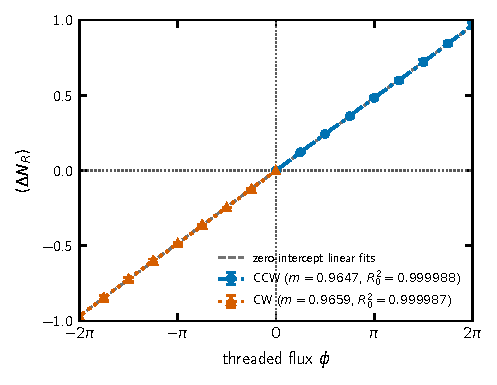
\includegraphics[width=0.96\columnwidth]{hard_wall_nshell1_flux_chirality_Nx32.pdf}
    \caption{\textbf{Hard-wall spectral chirality from monitored endpoints.}
    Trajectory-averaged right-half charge response for
    $N_x\times N_y=32\times24$, $n_{\rm shell}=1$, $\alpha_1=1$, and
    $\alpha_2=30$.  The hard walls lie at $x=8$ and $24$.  Each of the
    $S=100$ pure half-filled endpoint states was prepared for 48 raster-$y$
    cycles with perfect correction and no postselection; no monitored
    dynamics is rerun during the 256-interval spectral continuation.  Blue
    circles with a dash-dotted line show CCW threading, while orange triangles
    with a dotted line show CW threading.  Bars are pointwise trajectory SEMs
    and can be smaller than the markers.  Gray dashed segments are separate
    zero-intercept fits to $\langle\Delta N_R\rangle=m\phi/(2\pi)$; the
    slopes and through-origin $R_0^2$ values are given in the legend.  The
    horizontal coordinate omits the signed $10^{-7}$ branch regulator used in
    the numerical selector.  Total charge conservation gives
    $\Delta N_L=-\Delta N_R$, so the redundant left-half curve is not shown.}
    \label{fig:HardWallFluxChirality}
\end{figure}

A complementary endpoint diagnostic uses the modular Hamiltonian itself as a
generator.  For a half-cylinder cut $A(y_0)$ and trajectory $\xi$, let
$C_{A,\xi,y_0}$ be the restricted occupation matrix and
$G_{A,\xi,y_0}=2C_{A,\xi,y_0}-\mathbf{1}_A$.  The one-body modular generator is
\begin{equation}
 K_{A,\xi,y_0}
 =\log\!\left[(\mathbf{1}_A-C_{A,\xi,y_0})
 C_{A,\xi,y_0}^{-1}\right]
 =-2\operatorname{arctanh}G_{A,\xi,y_0}.
 \label{eq:EndpointModularGenerator}
\end{equation}
After placing a localized packet $\varphi_p(0)$ at one wall and one endpoint
of the half cylinder, we evolve it exactly in modular time,
\begin{equation}
 \varphi_{p,\xi,y_0}(t_{\rm mod})
 =e^{-\ii K_{A,\xi,y_0}t_{\rm mod}}\varphi_p(0).
 \label{eq:EndpointModularPacketEvolution}
\end{equation}
The signed observable $D_{p,\xi,y_0}(t_{\rm mod})$ is the continuous branch of
the packet's $y$ center-of-mass displacement relative to its initial value.
For the statistical reduction, we first average the 40 translated cut origins
within each trajectory and only then form the mean and SEM over the $S=10$
independent trajectories.

Figure~\ref{fig:HardWallModularChirality} applies this construction to the
cycle-50 $16\times40$ hard-wall covariance snapshots at
$n_{\rm shell}=1$.  Charge is initially localized at the two wall columns
$x=5,11$ and the two endpoints $y-y_0=0,19$ of the reduced half cylinder.
To keep the spatial information readable, we display only the diagonally
opposed pair initialized at $(x,y-y_0)=(5,0)$ and $(11,19)$.  The lower-left
packet develops positive displacement while the upper-right packet develops
negative displacement.  At $t_{\rm mod}=32$, their trajectory means are
\begin{equation}
 (\langle\Delta y\rangle_{(5,0)},
  \langle\Delta y\rangle_{(11,19)})=(8.016,-7.395),
 \label{eq:EndpointModularDisplacements}
\end{equation}
with SEMs $(0.643,0.601)$.  The complementary two corners, not plotted, have
the same endpoint-sign structure.  The density overlay shows the spatial
redistribution before this center-of-mass reduction.  The maximum saved charge
drift is $6.89\times10^{-15}$.

We use displacement rather than a finite-difference velocity because the
finite subsystem produces coherent oscillations in modular time; an
``instantaneous velocity'' would depend on an additional smoothing or fit
window.  We likewise do not average the unordered modular eigenvalues across
trajectories.  Chirality is encoded in the oriented modular eigenvectors (or,
with translation symmetry, in a momentum-resolved dispersion), not in the
scalar eigenvalue density alone.  The signed packet motion therefore supplies
the more direct diagnostic available in the saved data.  As with the flux
calculation, modular time is not the monitored circuit clock.  Figure
\ref{fig:HardWallModularChirality} is evidence for the handed entanglement
dynamics of the prepared endpoint ensemble, not a measurement of real-time
charge propagation under the adaptive circuit.

\begin{figure*}[t]
    \centering
    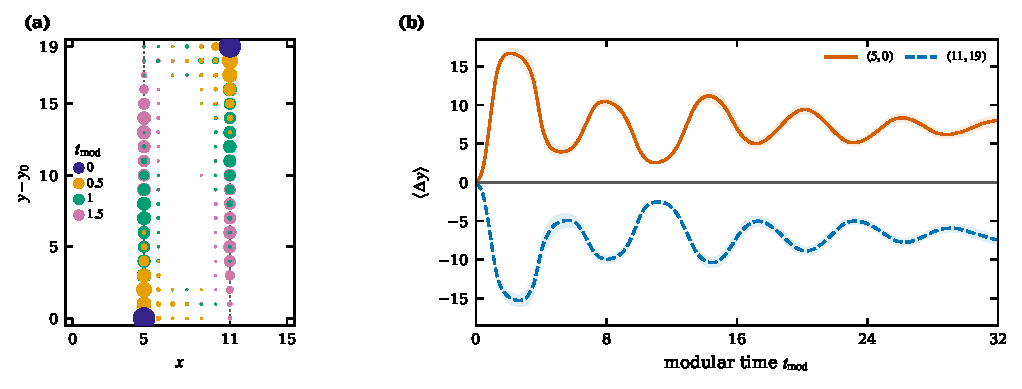
\includegraphics[width=0.98\textwidth]{modular_charge_chirality_cycle50_nsh1.pdf}
    \caption{\textbf{Modular charge propagation from monitored hard-wall
    endpoints.}  Panel (a) overlays two independently evolved modular packet
    densities at $t_{\rm mod}=0,0.5,1,1.5$ for the cycle-50,
    $N_x\times N_y=16\times40$, $n_{\rm shell}=1$ hard-wall endpoint
    ensemble.  The two packets start at the bottom-left corner $(5,0)$ and the
    top-right corner $(11,19)$.  Purple, orange, green, and pink identify the
    four modular times, respectively.  The circles are opaque with edges matched
    to their fills; marker area scales as the square root of local packet
    density.  Gray dotted lines mark the physical wall columns $x=5$ and $11$.
    The spatial overlay uses the saved modular
    generator constructed after averaging the ten samples and 40 translated
    origins.  Panel (b) gives the statistically primary signed
    center-of-mass displacement: the 40 translated origins are first averaged
    inside each trajectory, after which curves and shaded bands show the mean
    and $\pm$SEM over $S=10$ independent trajectories.  Only the same two
    diagonal corners are retained: the solid orange curve is $(5,0)$ and the
    dashed blue curve is $(11,19)$.  Their opposite displacement signs give the modular
    handedness.  Evolution is the exact spectral exponential in
    Eq.~\eqref{eq:EndpointModularPacketEvolution}; $t_{\rm mod}$ is modular
    time, not monitored circuit time.}
    \label{fig:HardWallModularChirality}
\end{figure*}

\begingroup
\raggedbottom
\subsection{Trajectory Averaged Dynamics}
\label{sec:TrajectoryAveragedDynamics}

We now ask which boundary signatures remain when the measurement record is
discarded.  Using the measurement-feedback Kraus operators defined above,
the elementary quantum channel is
\begin{equation}
 \mathcal E_{t,i,\sigma}(\hat\rho)
 =\sum_{\xi=0,1}\hat K_{t,i,\sigma}(\xi)\hat\rho
 \hat K_{t,i,\sigma}^{\dagger}(\xi).
 \label{eq:ElementaryAveragedChannel}
\end{equation}
No additional Born weight multiplies these terms: the trace of each
unnormalized Kraus branch already gives its outcome probability.
For the schedule $\mathcal S$ of Eq.~\eqref{eq:AdaptiveCycleKraus}, one
complete cycle is the product channel
\begin{align}
 \mathcal E_{\mathrm{cyc},\mathcal S}
 &=\prod_{t=1}^{T}\mathcal E_{t,i_t,\sigma_t}
 \nonumber\\
 &\equiv\mathcal E_{T,i_T,\sigma_T}\cdots
 \mathcal E_{2,i_2,\sigma_2}\mathcal E_{1,i_1,\sigma_1},
 \label{eq:ProductAveragedChannel}
\end{align}
where the product denotes composition of channels, not a tensor product,
and the rightmost ($t=1$) channel acts first.  Thus
\begin{equation}
 \mathcal E_{\mathrm{cyc},\mathcal S}(\hat\rho_0)
 =\sum_{\boldsymbol\xi}p(\boldsymbol\xi)
 \hat\rho_{\boldsymbol\xi},
 \label{eq:CycleChannelBornAverage}
\end{equation}
with exactly the record probabilities and conditioned states in
Eqs.~\eqref{eq:AdaptiveRecordProbability} and
\eqref{eq:AdaptiveConditionalState}.  Successive cycles compose in the same
order; if the schedule repeats, the $n$-cycle channel is simply
$\mathcal E_{\mathrm{cyc},\mathcal S}^{\,n}$.  When schedules change, we keep
their ordered product and average only the measurement outcomes, not the
schedule choices.  Writing $\overline{\hat\rho}(n)$ for the resulting
Born-weighted state, its two-point function is
\begin{equation}
 \overline C_{ij}(n)
 =\operatorname{Tr}\!\left[\overline{\hat\rho}(n)
 \hat c_i^\dagger\hat c_j\right].
 \label{eq:TrajectoryAveragedCorrelation}
\end{equation}
Here $C$ is the occupation matrix of
Eq.~\eqref{eq:ComplexCovarianceDefinition}, not the centered covariance
$G=2C-\mathbf{1}$.  The sum over records in
Eq.~\eqref{eq:CycleChannelBornAverage} need not be evaluated by sampling
trajectories.  In fact, each elementary channel can be written exactly as
$\mathcal E_{i,\sigma}=\mathrm{Id}+\mathcal L_{i,\sigma}$, where
\begin{align}
 \mathcal L_{i,-}
 &=\mathcal D[\hat\chi_{i,-}^{\dagger}]
   +\mathcal D[\hat{\mathcal N}_{i,-}],\nonumber\\
 \mathcal L_{i,+}
 &=\mathcal D[\hat\chi_{i,+}]
   +\mathcal D[\hat{\mathcal N}_{i,+}],
 \label{eq:ElementaryChannelLindbladian}
\end{align}
and
\begin{equation}
 \mathcal D[\hat L](\hat\rho)
 =\hat L\hat\rho\hat L^\dagger
 -\tfrac12\{\hat L^\dagger\hat L,\hat\rho\}.
 \label{eq:AveragedChannelDissipator}
\end{equation}
The first term implements gain or loss, and the second is the number
dephasing associated with the occupation measurement.  This is an exact
identity for the finite measurement-feedback reset, not a small-time
approximation to $e^{\mathcal L_{i,\sigma}}$.

For $j=(i,\sigma)$, use the projector $P_j$ and complement $Q_j$ of
Eq.~\eqref{eq:StoredOWProjector}, and set $s_-=1$, $s_+=0$.  The induced
increment of the occupation matrix closes as
\begin{align}
 \Delta_j\overline C
 &=s_\sigma P_j-\{P_j,\overline C\}
   +P_j\overline C P_j,\nonumber\\
 \overline C'
 &=Q_j\overline C Q_j+s_\sigma P_j.
 \label{eq:ExactMeanChannelCovarianceUpdate}
\end{align}
Equivalently, the centered covariance obeys
\begin{equation}
 \overline G'=Q_j\overline GQ_j+(2s_\sigma-1)P_j.
 \label{eq:ExactMeanChannelCenteredUpdate}
\end{equation}
These relations hold without a Gaussian closure assumption.  They are the
updates implemented by the canonical CPU routine
\texttt{run\_markov\_channel} with perfect correction and number dephasing
enabled.  Applying them in the prescribed order computes the Born-averaged
two-point dynamics exactly, up to numerical roundoff, without sampling
measurement outcomes or storing a many-body density matrix.  The
noncommuting product retains the full finite-step ordering; replacing it
by continuous evolution under $\sum_j\mathcal L_j$ would define a
different dynamics.

For the spectrum, we then average $\overline C$ over translations along
$y$ before diagonalizing each momentum block.  Figure~\ref{fig:HardWallMeanChannel}(a)
shows the hard-wall spectrum at a cycle-boundary steady state of this
fixed ordered channel.  At $\alpha_1=1$, branches extend
between the nearly empty and filled bands, whereas the $\alpha_1=3$
control remains close to occupations zero and one.  The intermediate
branches have occupations approximately $0.5466$ near $k_y=0$;
exact half occupation at that momentum is not imposed in the comparison.

Panel~(b) applies the squared-correlator estimator of
Eq.~\eqref{eq:EndpointSquaredCorrelator} to $\overline C$ itself:
$C_{\overline G}^{\mathrm{av}}(r_y)$ denotes the full-$x$ average of
$\sum_{y,\mu,\nu}|\overline C_{(x,y,\mu),(x,y+r_y,\nu)}|^2/(2N_y)$.
The Born average precedes squaring, unlike
$\overline{C_G^{\mathrm{av}}}$ in Fig.~\ref{fig:HardWallCorrelatorSummary}.
Both curves fall below $10^{-8}$ by $r_y=5$; no decay law is fitted.
Since the averaged state need not be Gaussian, this squared two-point
function is not identified with its connected density correlator.

\begin{center}
    \begin{minipage}{\columnwidth}
    \centering
    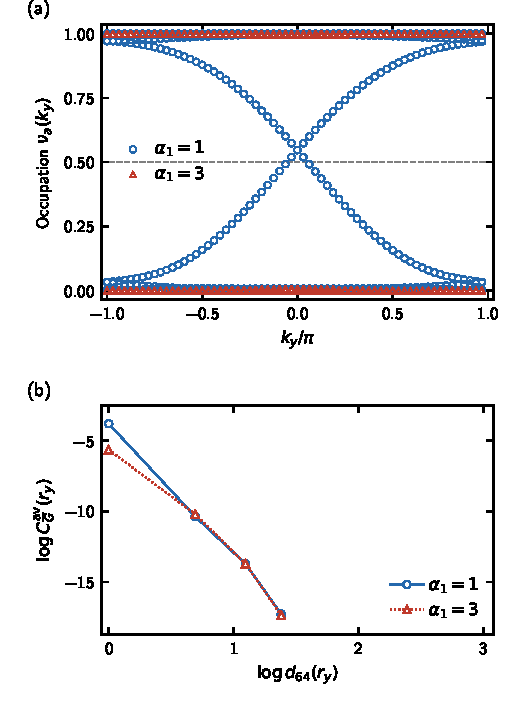
\includegraphics[width=\columnwidth]{hard_wall_mean_channel_summary_2x1.pdf}
    \begin{minipage}{0.96\columnwidth}
        \captionof{figure}{\textbf{Trajectory-averaged hard-wall spectrum and correlations.}
        Blue circles and red triangles denote $\alpha_1=1$ and $3$, respectively,
        with $\alpha_2=30$, $N_x=20$, $N_y=64$, and $n_{\rm shell}=1$.
        This complementary channel calculation uses maximally mixed
        initialization, perfect correction, and the inclusive slab
        $x=5,\ldots,15$; measurements act in all slabs, with OW support
        truncated at the interfaces.  Outcomes are averaged analytically,
        rather than sampled over $S$ independent trajectories.
        The within-cell
        order is $(A,+),(A,-),(B,+),(B,-)$, as in the trajectory
        simulations; the site order is fixed raster-$y$ in every cycle.
        Both panels use the endpoint at cycle $128=2N_y$.
        (a) Occupation spectrum after translation averaging along $y$;
        all 40 modes per momentum, including exterior modes, are retained.
        The dashed line marks occupation $1/2$.
        (b) Full-$x$ average of the squared Born-averaged two-point function
        versus chord distance, with natural logarithms on both axes.
        Here squaring precedes the spatial origin average; no spatial
        twirl is applied first.  The $10^{-8}$ display cutoff, as in
        Fig.~\ref{fig:HardWallCorrelatorSummary}, leaves $r_y=1,\ldots,4$
        visible out of $1,\ldots,N_y/2$; it is not a certified numerical
        floor.  Lines in (b) only guide the eye.  For both alphas,
        the last ten cycle-to-cycle changes satisfy
        $\|\Delta\overline C\|_{\rm F}/\sqrt{2N_xN_y}<10^{-12}$.
        There is no
        temporal or schedule average, fit, or sampling error bar.}
        \label{fig:HardWallMeanChannel}
    \end{minipage}
    \end{minipage}
\end{center}

The closest comparison is the dissipatively prepared correlation spectrum
in Fig.~3 of Goldstein~\cite{Goldstein2019}, which likewise exhibits
intermediate-occupation boundary branches.  For Gaussian mixed states,
these spectra also determine a quadratic modular Hamiltonian, whose
boundary modes can be probed through full counting
statistics~\cite{MaoZhaiYang2025}.  Our Born-weighted average need not be
Gaussian, so we interpret Fig.~\ref{fig:HardWallMeanChannel}(a) as a
single-particle boundary signature, not as the full many-body modular
spectrum or a demonstration of quantized transport.  The distinction for
the adaptive algorithm is that retaining the record gives access to the
conditional boundary-state ensemble studied above: its entropy and charge
observables are formed within each trajectory before averaging, and are
not observables of $\overline{\hat\rho}$.  Thus, preparing the
record-resolved ensemble does not require the unconditional mixture to
become pure.

\clearpage
\endgroup
\bibliographystyle{apsrev4-2}
\IfFileExists{references.bib}
    {\bibliography{references}}
    {\bibliography{technical_report/references}}


\end{document}
